%
% Template for DAS course projects
%
\documentclass[a4paper,11pt,oneside]{book}
\usepackage[latin1]{inputenc}
\usepackage[english]{babel}
\usepackage{amsfonts}
\usepackage{amsmath}
\usepackage{bm}
\usepackage{amssymb,amsmath,color}
\usepackage{cite}
\usepackage{graphicx}
\usepackage{float}
\usepackage{caption}
\usepackage{subcaption}
\usepackage[hidelinks]{hyperref}
\usepackage{cleveref}
\usepackage{booktabs}

\begin{document}
\pagestyle{myheadings}

\def\N{{\mathbb{N}}}
\def\R{{\mathbb{R}}}
\def\z{{\bm{z}}}
\def\Q{{\bm{Q}}}
\def\r{{\bm{r}}}
\def\p{{\bm{p}}}


%%%%%%%%%%% Cover %%%%%%%%%%%
\thispagestyle{empty}                                                 
\begin{center}                                                            
    \vspace{5mm}
    {\LARGE UNIVERSIT\`A DI BOLOGNA} \\                       
      \vspace{5mm}
\end{center}
\begin{center}
  
\includegraphics[scale=.27]{figs/logo_unibo}
\end{center}
\begin{center}
      \vspace{5mm}
      {\LARGE School of Engineering} \\
        \vspace{3mm}
      {\Large Master Degree in Artificial Intelligence} \\
      \vspace{20mm}
      {\LARGE Distributed Autonomous Systems} \\
      \vspace{5mm}{\Large\textbf{TITLE}}                  
      \vspace{15mm}
\end{center}
\begin{minipage}{0.48\linewidth}
      \raggedright
     {\large Professors:}\\
     \textbf{Giuseppe Notarstefano} \\
     \textbf{Ivano Notarnicola} \\        
%      \vspace{13mm}
\end{minipage}
\begin{minipage}{0.48\linewidth}
      \raggedleft
      {\large Students:}\\
      \textbf{\@ Valerio Costa} \\
      \textbf{\@ Tian Cheng Xia} \\  
\end{minipage}
\begin{center}
\vfill
      {\large Academic year \@2024/2025} \\
\end{center}



\newpage
\thispagestyle{empty}

%%%%%%%%%%% Abstract %%%%%%%%%%%%
\begin{center}
\chapter*{}
\thispagestyle{empty}
{\Huge \textbf{Abstract}}\\
\vspace{15mm}
\end{center}

\tableofcontents \thispagestyle{empty}
% \listoffigures\thispagestyle{empty}

%%%%%%%%%% Introduction %%%%%%%%%%
\chapter*{Introduction}
\addcontentsline{toc}{chapter}{Introduction}

\section*{Motivations} 

The project aims at solving and implementing distributed algorithms to solve two specific tasks. The first one, which can be solved using the gradient tracking algorithm, involves the problem of distributed target localization where some tracking robots want to estimate the position of some targets for which only noisy measurements are known. The second one, which is an aggregative optimization problem, consists of positioning robots balancing the requirements of being close to private targets while keeping the whole fleet tight. For both tasks, we experiment the resulting implementation to assess their results in terms of correctness, convergence, and scalability.

The rest of the report is structured as follows: in \Cref{ch:quadratic}, we implement the gradient tracking algorithm for quadratic functions. In \Cref{ch:localization}, we solve and show the results for the task of target localization. In \Cref{ch:aggregative}, we present the solution and the experiments for the task of robots positioning.


\section*{Contributions}

This project provides a small comparison benchmark of some distributed algorithms. These results, although limited, show the effectiveness of these algorithms in solving some tasks for which taking a centralized approach is not realistic. 

In practical terms, most of the work has been done in pair programming and both group members have contributed equally to the implementation.




% \chapter{Multi-Robot Target Localization}

\setcounter{page}{1}
\chapter{Gradient tracking with quadratic functions} \label{ch:quadratic}


\section{Problem definition}

The first task aim is to solve a multi-robot target localization problem. Indeed, we consider a fleet of $N \in \N$ agents and a collection of $N_T \in \N$, in which each agent makes noisy measurements of its distance from every target. The objective is to design a distributed algorithm, in order to minimize the loss between every target estimated position and its ground truth (as formulated below), with a particular focus on trying to reach a consensus within the fleet.

\[
      \min_{\z \in \R^{d}} \sum_{i=1}^{N} l_i(\z)
\]


The first part of the task consists of implementing the gradient tracking algorithm generalized in $\R^d$ and then experiment with the implementation using quadratic functions, which we define in the usual way as:
\[
      f(\z) = \frac{1}{2} \z^T \Q \z + \r^T \z
      \quad
      \nabla f(\z) = \Q \z + \r
\]
where $\z \in \R^{d}$, $\Q \in \R^{d \times d}$ is positive definite, and $\r \in \R^{d}$.

\section{Code structure}
The code provided is structured with the following main modules:
\begin{description}
      \item[algorithm.py] Two functions, allowing to run the distributed gradient tracking algorithm and its centralized version.
      \item[loss.py] Class definition of the quadratic loss function.
      \item[plot.py] All the functions used to plot the loss, gradient norm and  distance to optimum evolution over iterations.
      \item[scenarios.py] Two functions, one aiming to create the graph $G$ and the relative adjacency matrix $A$, while the other designed to initialize the parameters and the quadratic loss functions.
      \item[utils.py] The definition of the functions for computing the average estimate error for each agent with respect to its ground truth, and the average consensus error meaning the average distance of each agent estimate with the consensus. 
\end{description}
In practice all the experiments can be executed from the script \texttt{main\_quadratic.py}.


\section{Experiments}


We analyzed the behavior with quadratic functions through the definition of different problems with different kinds of graph patterns (in particular complete, binomial, cycle, star, and path graph). The configurations we tested are the following:
\begin{itemize}
      \item A small problem ($5$ agents in $\R^3$),
      \item A problem with higher dimensionality ($5$ agents in $\R^{15}$),
      \item A problem with many agents ($15$ agents in $\R^3$), and
      \item A problem with many agents in higher dimensionality ($15$ agents in $\R^{15}$).
\end{itemize}
In addition, we performed a comparison between the distributed gradient tracking algorithm and the centralized one. For compactness in the discussion, in the rest of this report we show the results with a single initialization seed and, if not specified, it indicates that the results are consistent across different initializations. Also, for readability, for quadratic functions we report the distance to the optimum in semi-logarithmic scale instead of the cost itself which can be negative.


\subsection{Comparison between different graph patterns}

For the starting small problem, we can observe from \Cref{fig:quadratic_5_3} a relatively smooth improvement of the cost function and an exponentially decreasing gradient in all cases. Moreover, a result that can be expected and is consistently persistent in all the other experiments is that consensus is reached slightly faster with a complete graph. Next, by experimenting with higher dimensionality, we can observe from \Cref{fig:quadratic_5_15} that the behavior of both the cost and its gradient are very similar to the previous case with the only difference that more iterations are required to reach full convergence, indicating that the dimensionality is marginal in changing the difficulty of the problem. 

\begin{figure}[H]
      \centering
      \begin{subfigure}[t]{0.46\linewidth}
            \centering
            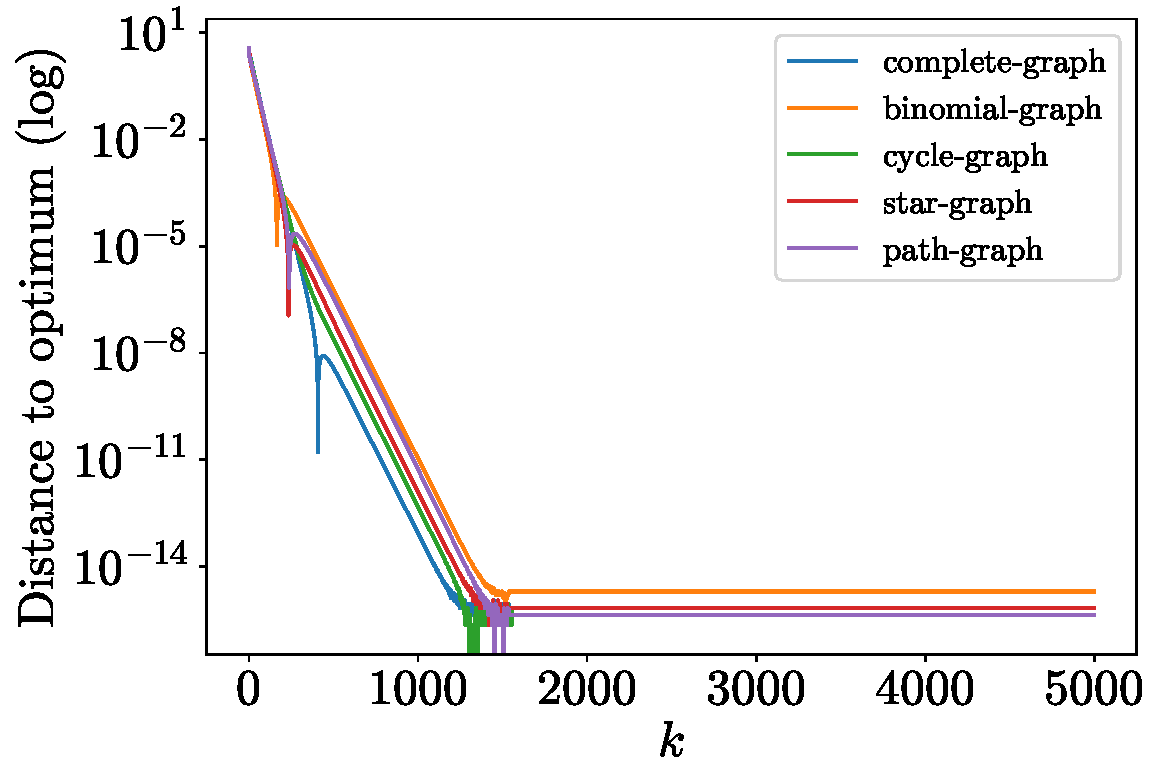
\includegraphics[width=\linewidth]{./figs/quadratic/5_3/distance.pdf} 
            \caption{Distance to optimum}
      \end{subfigure}
      \hfill
      \begin{subfigure}[t]{0.46\linewidth}
            \centering
            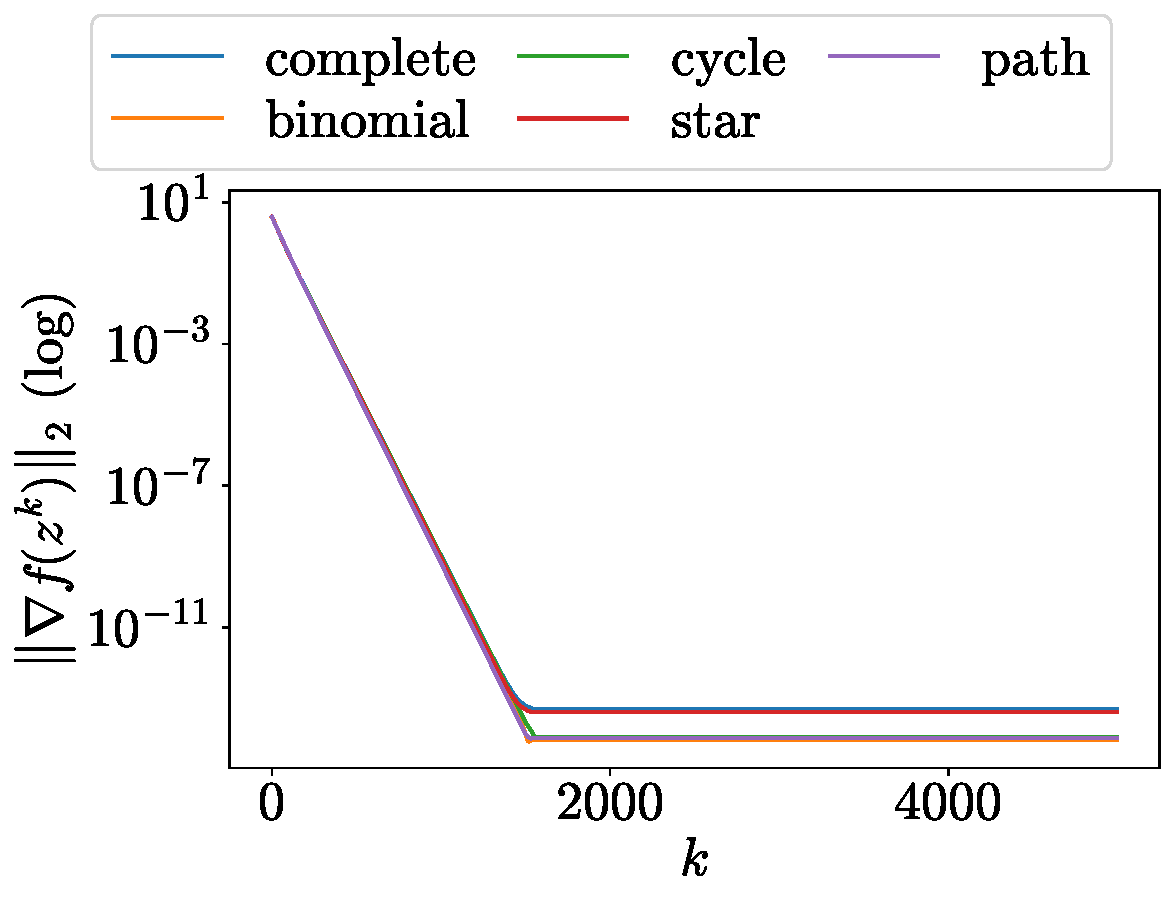
\includegraphics[width=\linewidth]{./figs/quadratic/5_3/gradient.pdf} 
            \caption{Gradient norm evolution}
      \end{subfigure}
      \hfill
      \begin{subfigure}[t]{0.46\linewidth}
            \centering
            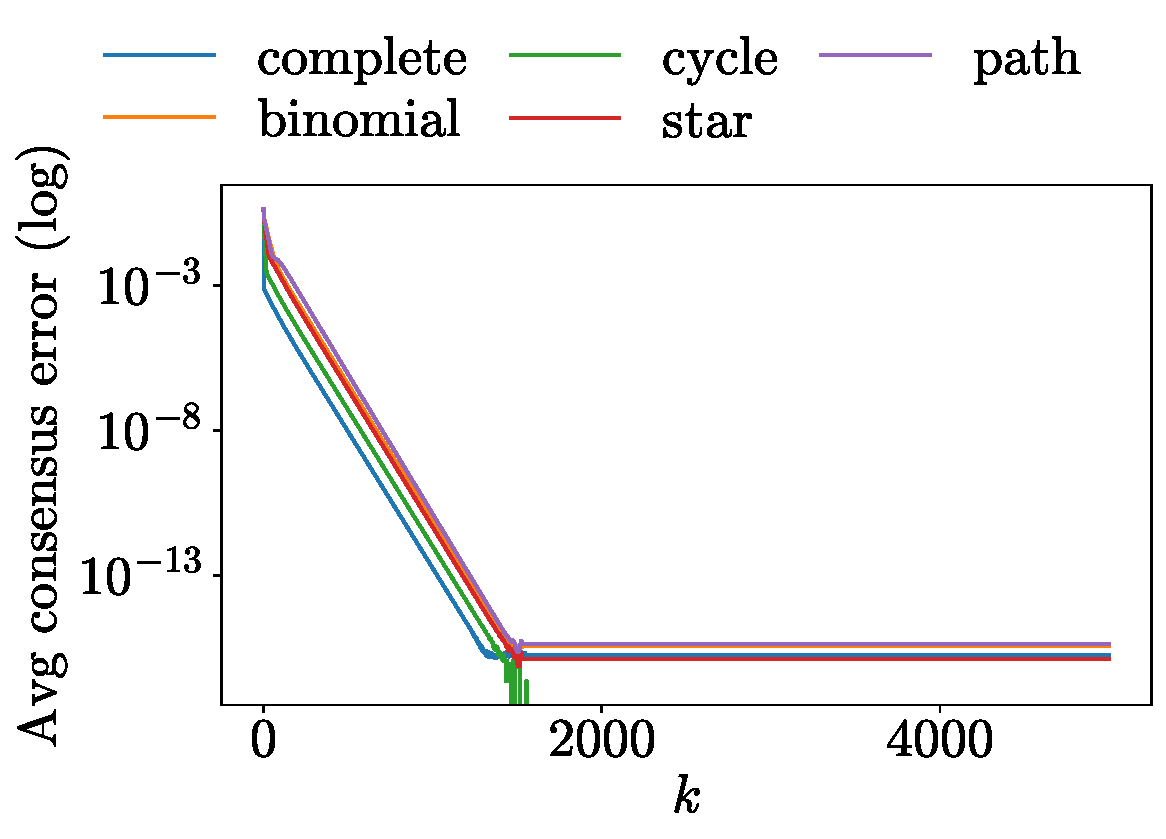
\includegraphics[width=\linewidth]{./figs/quadratic/5_3/consensus.pdf} 
            \caption{Consensus error}
      \end{subfigure}
      \caption{Quadratic function minimization with $5$ agents in $\R^{3}$}
      \label{fig:quadratic_5_3}
\end{figure}

\begin{figure}[H]
      \centering
      \begin{subfigure}[t]{0.46\linewidth}
            \centering
            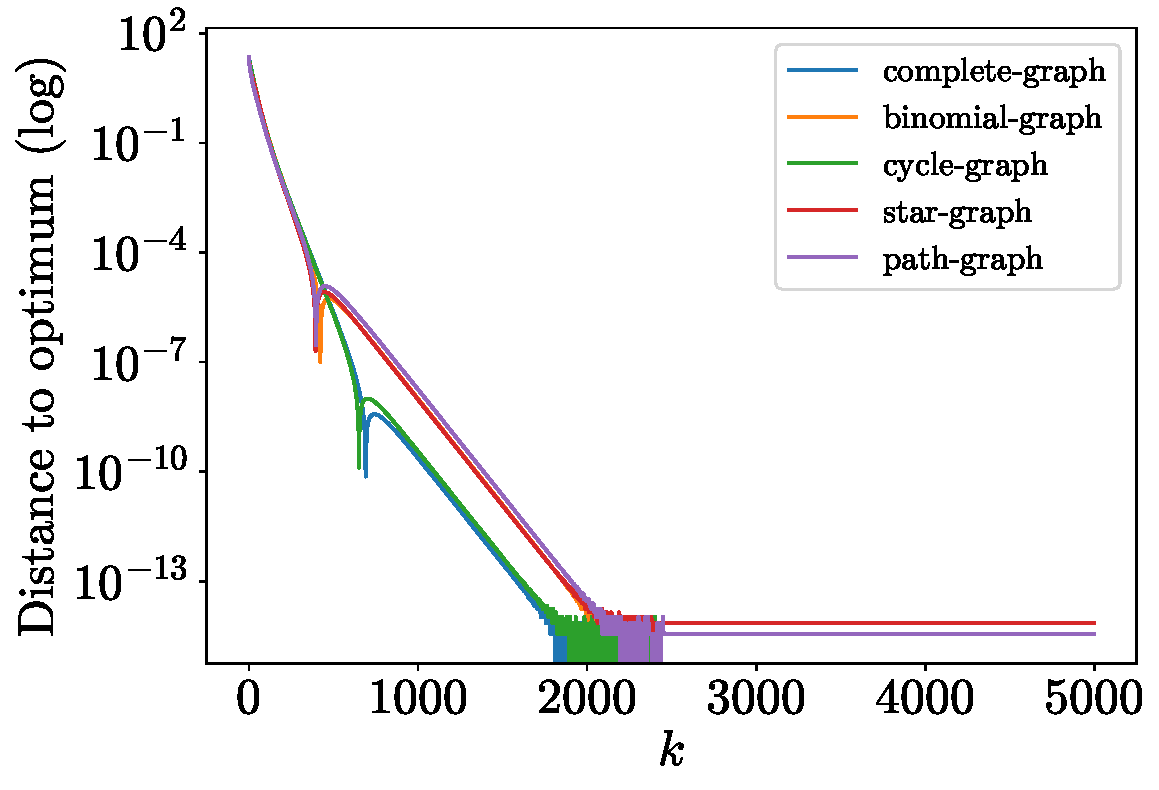
\includegraphics[width=\linewidth]{./figs/quadratic/5_15/distance.pdf} 
            \caption{Cost evolution}
      \end{subfigure}
      \hfill
      \begin{subfigure}[t]{0.46\linewidth}
            \centering
            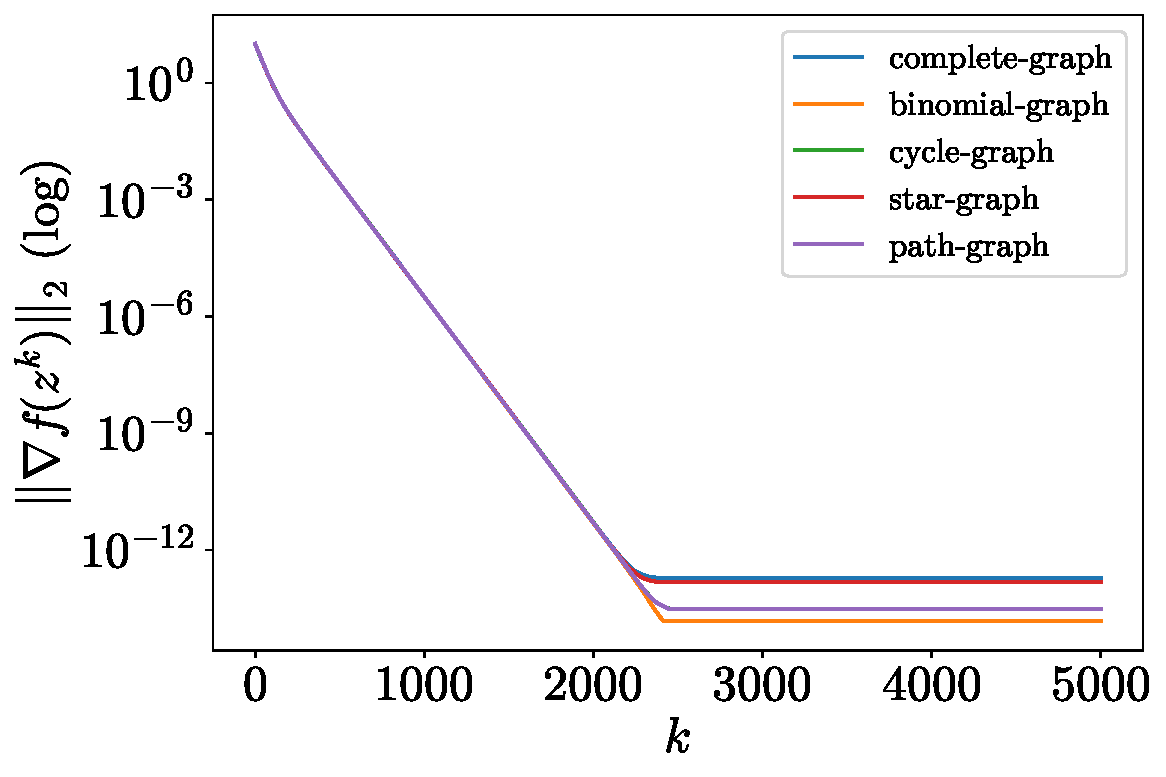
\includegraphics[width=\linewidth]{./figs/quadratic/5_15/gradient.pdf} 
            \caption{Gradient norm evolution}
      \end{subfigure}
      % \hfill
      % \begin{subfigure}[t]{0.46\linewidth}
      %       \centering
      %       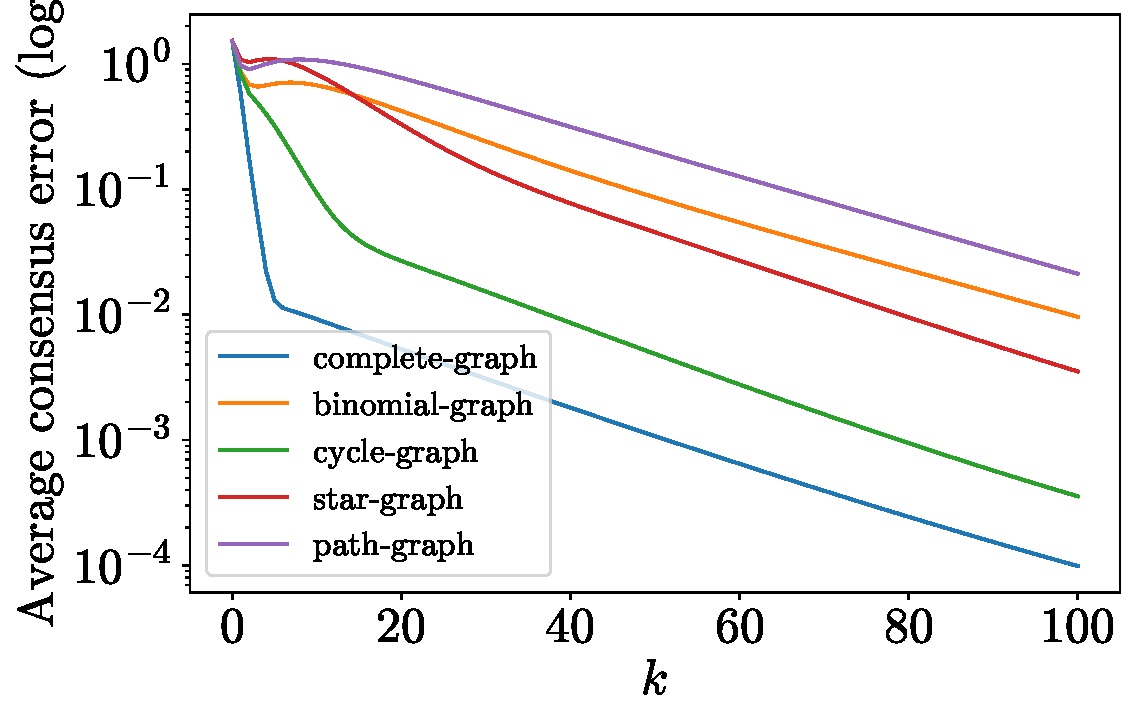
\includegraphics[width=\linewidth]{./figs/quadratic/5_15_100/consensus.pdf} 
      %       \caption{Consensus error}
      % \end{subfigure}
      \caption{Quadratic function minimization with $5$ agents in $\R^{15}$}
      \label{fig:quadratic_5_15}
\end{figure}

In the case of many agents with lower dimensionality, we can observe from \Cref{fig:quadratic_15_3} that the cost function does not reach the optimum within the given number of iterations with the configuration using the path graph, indicating that connectivity is important for larger numbers of agents. This can be explained by the fact that, by adding more agents, the overall problem includes more local losses and becomes more difficult to solve in a distributed way. From \Cref{fig:quadratic_15_15}, we observe the same convergence behavior as in the previous case and also confirm that, with higher dimensionality, the problem is not significantly affected.


% Follo
% The following plots represent how the behavior of the algorithm changes between different kinds of networks.

% and higher dimensionality In particular, we observed a much relevant change in terms of iterations required to reach convergence for the case with 15 agents, which needed an extension in the number of iterations to show when i t
% reaches equiili

\begin{figure}[H]
      \centering
      \begin{subfigure}[t]{0.46\linewidth}
            \centering
            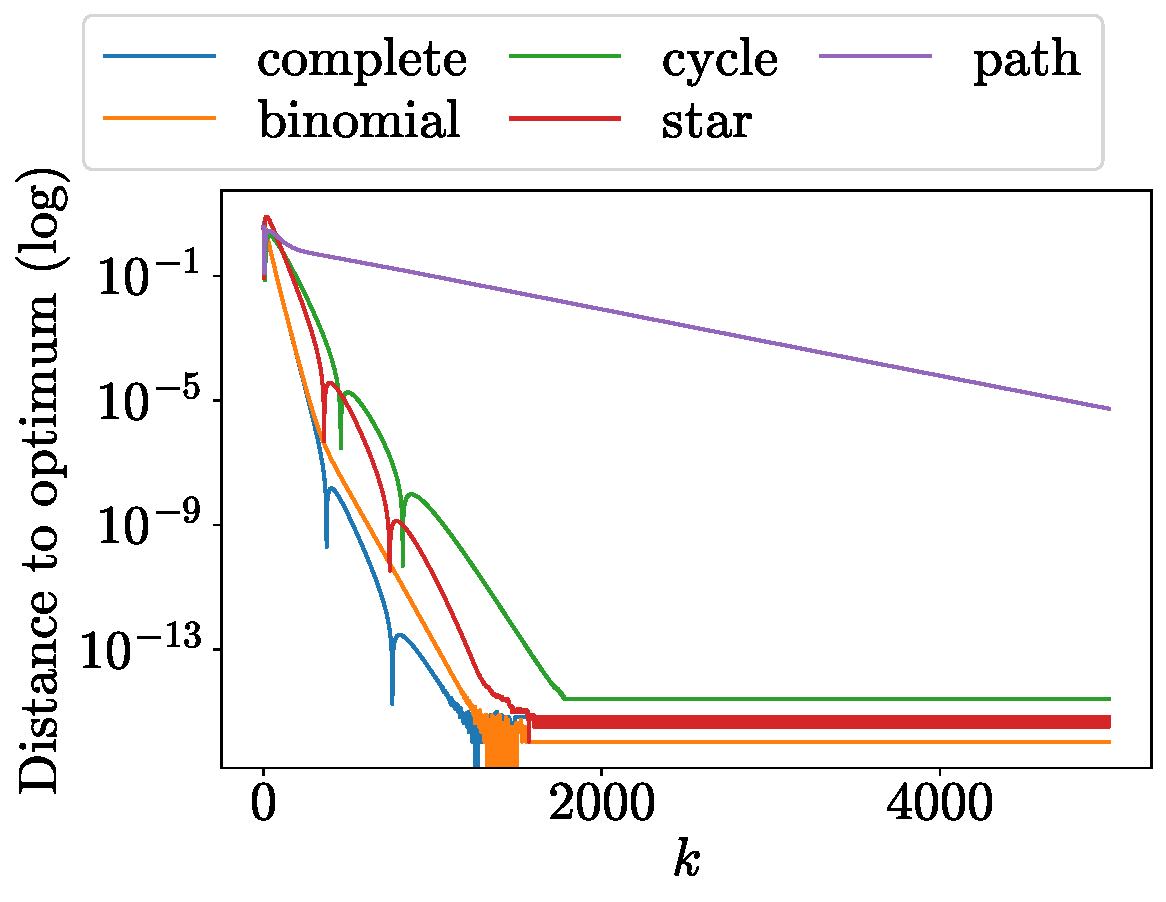
\includegraphics[width=\linewidth]{./figs/quadratic/15_3/distance.pdf} 
            \caption{Cost evolution}
      \end{subfigure}
      \hfill
      \begin{subfigure}[t]{0.46\linewidth}
            \centering
            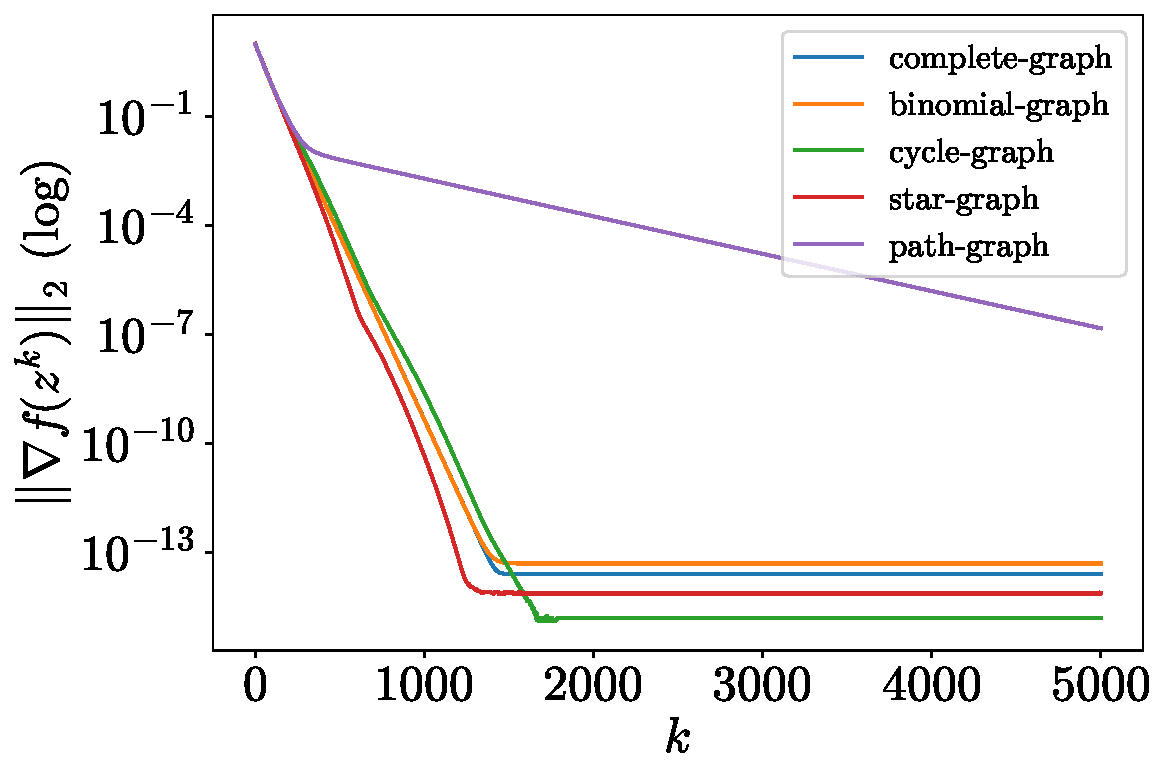
\includegraphics[width=\linewidth]{./figs/quadratic/15_3/gradient.pdf} 
            \caption{Gradient norm evolution}
      \end{subfigure}
      % \hfill
      % \begin{subfigure}[t]{0.46\linewidth}
      %       \centering
      %       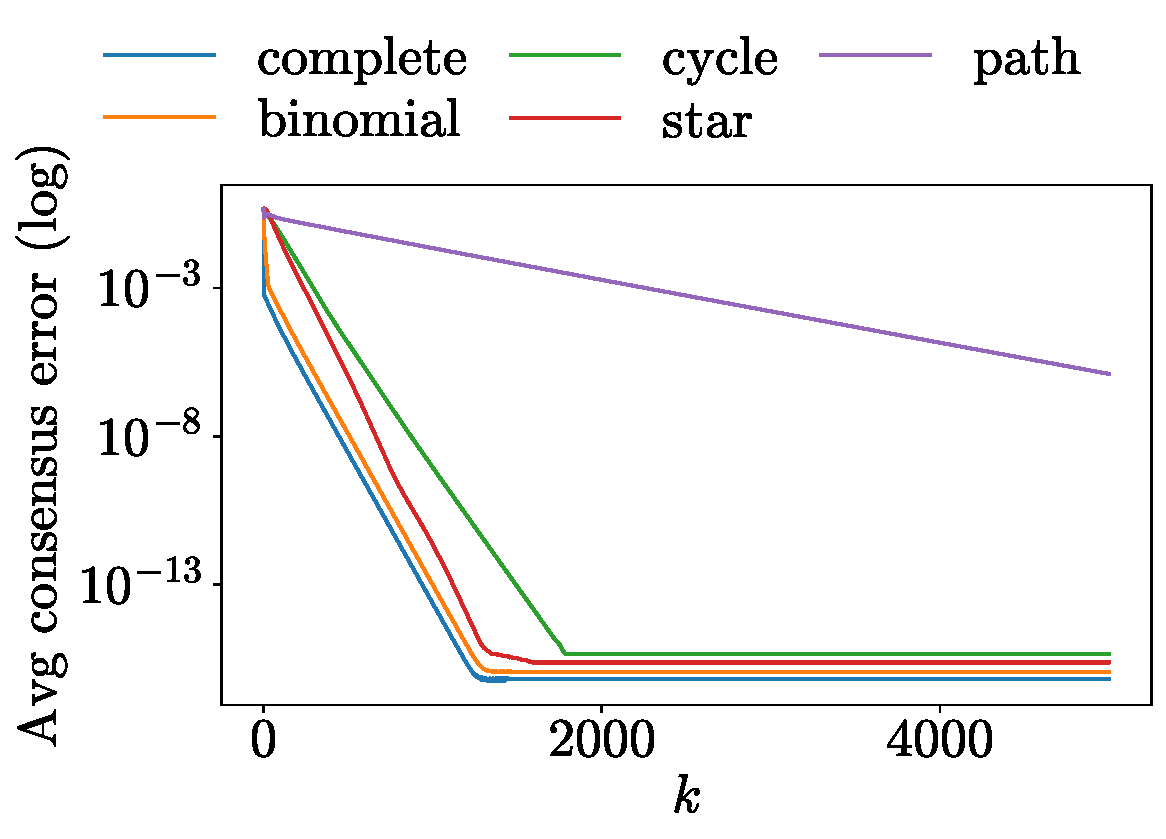
\includegraphics[width=\linewidth]{./figs/quadratic/15_3/consensus.pdf} 
      %       \caption{Consensus error}
      % \end{subfigure}
      \caption{Quadratic function minimization with $15$ agents in $\R^{3}$}
      \label{fig:quadratic_15_3}
\end{figure}

\begin{figure}[H]
      \centering
      \begin{subfigure}[t]{0.46\linewidth}
            \centering
            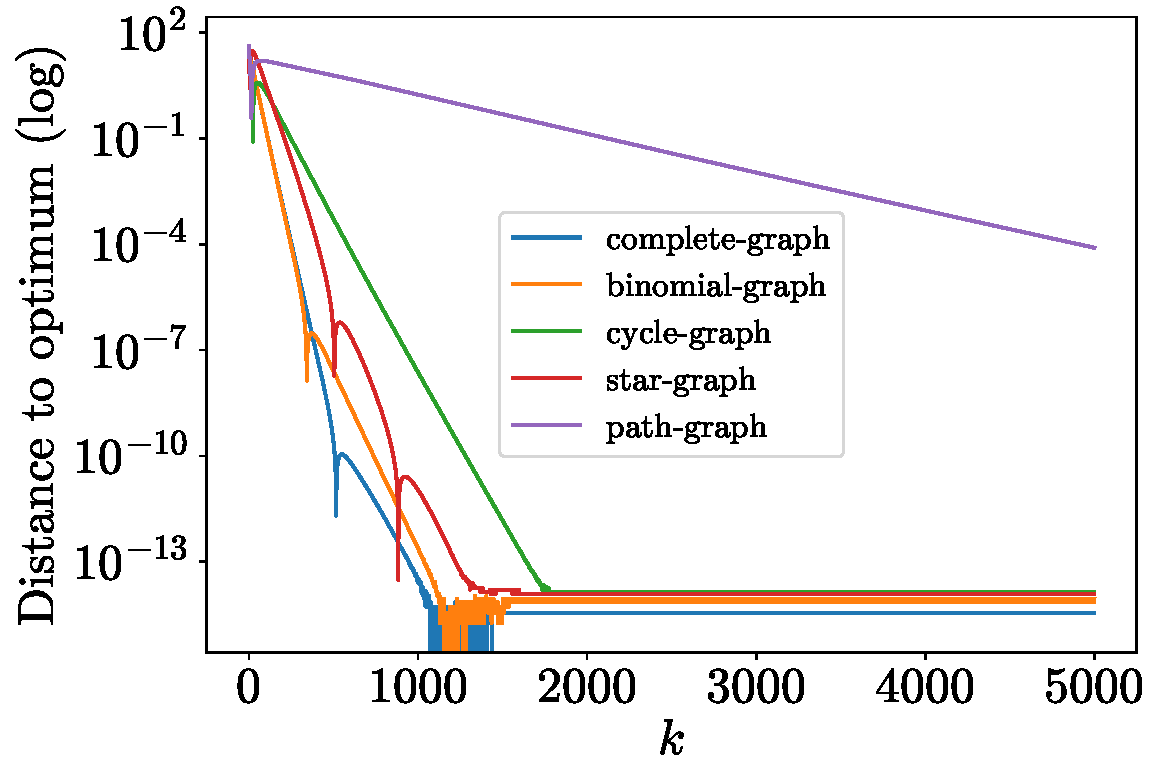
\includegraphics[width=\linewidth]{./figs/quadratic/15_15/distance.pdf} 
            \caption{Cost evolution}
      \end{subfigure}
      \hfill
      \begin{subfigure}[t]{0.46\linewidth}
            \centering
            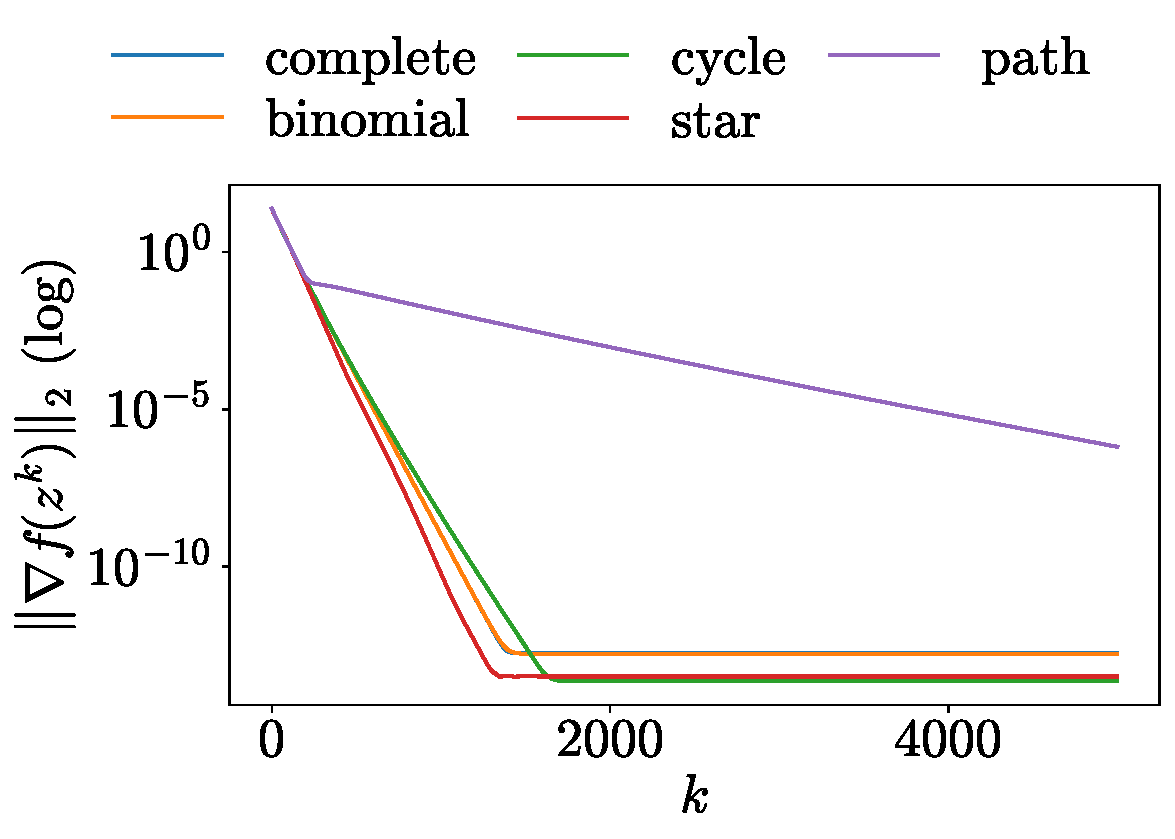
\includegraphics[width=\linewidth]{./figs/quadratic/15_15/gradient.pdf} 
            \caption{Gradient norm evolution}
      \end{subfigure}
      % \hfill
      % \begin{subfigure}[t]{0.46\linewidth}
      %       \centering
      %       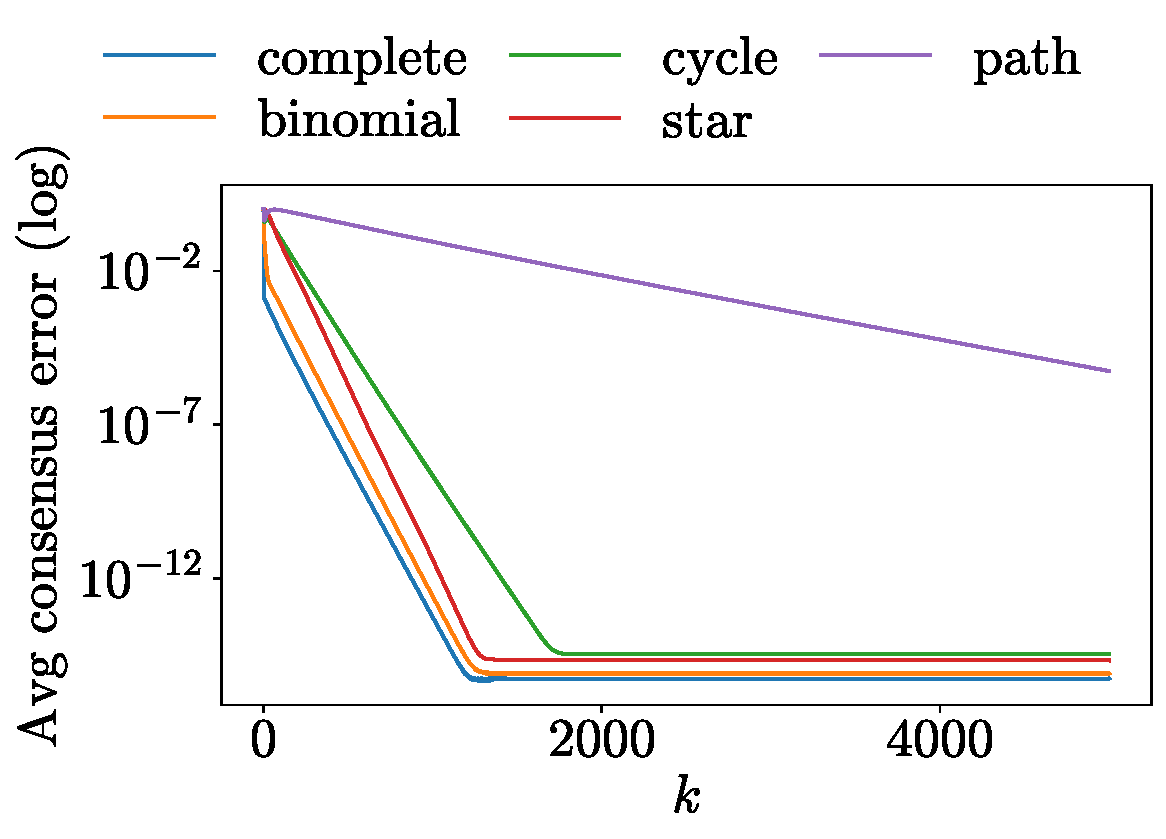
\includegraphics[width=\linewidth]{./figs/quadratic/15_15/consensus.pdf} 
      %       \caption{Consensus error}
      % \end{subfigure}
      \caption{Quadratic function minimization with $15$ agents in $\R^{15}$}
      \label{fig:quadratic_15_15}
\end{figure}


% At last, we experimented with a higher number of iterations to analyze the behavior at convergence. From \Cref{fig:quadratic_15_3_1000}, we can observe that the configuration with a complete graph is the one that converges with the most precise gradient, while the worst performing is the path graph that is the slowest to converge.

% \begin{figure}[H]
%       \centering
%       \begin{subfigure}[t]{0.46\linewidth}
%             \centering
%             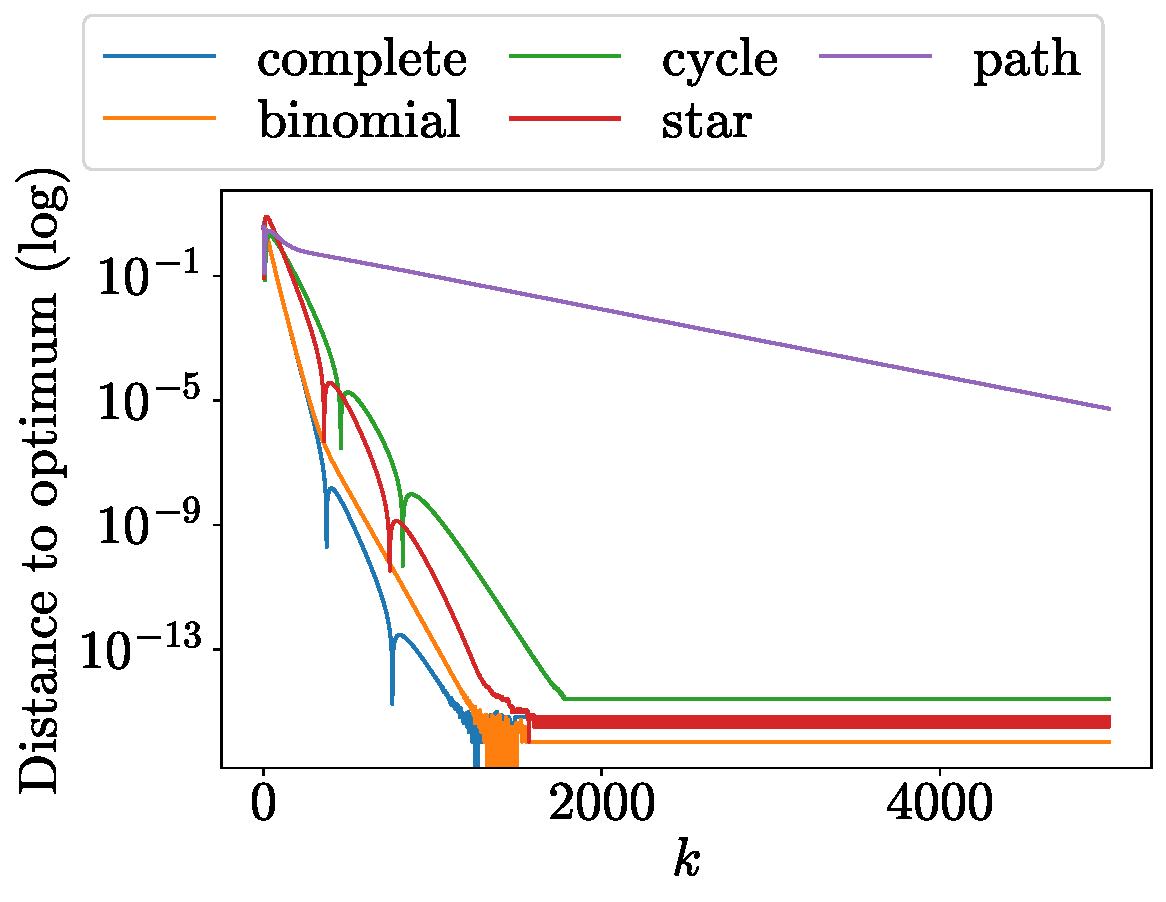
\includegraphics[width=\linewidth]{./figs/quadratic/15_3/distance.pdf} 
%             \caption{Cost evolution}
%       \end{subfigure}
%       \hfill
%       \begin{subfigure}[t]{0.46\linewidth}
%             \centering
%             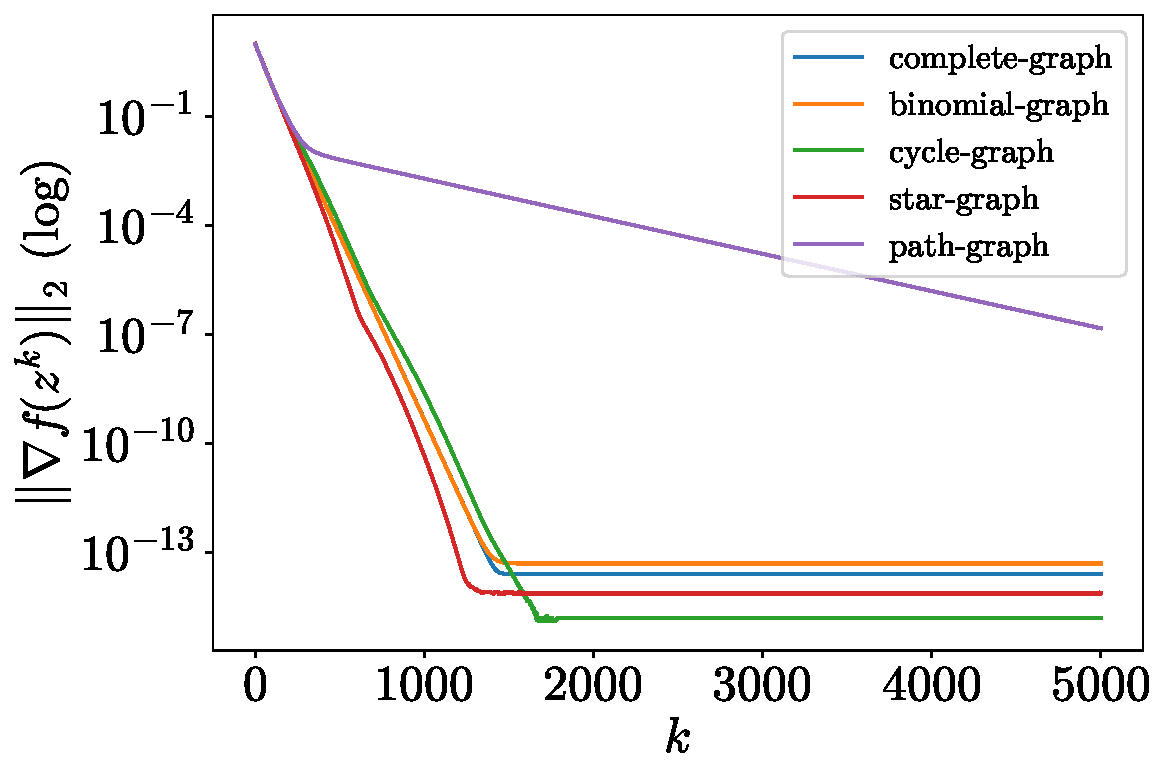
\includegraphics[width=\linewidth]{./figs/quadratic/15_3/gradient.pdf} 
%             \caption{Gradient norm evolution}
%       \end{subfigure}
%       % \hfill
%       % \begin{subfigure}[t]{0.46\linewidth}
%       %       \centering
%       %       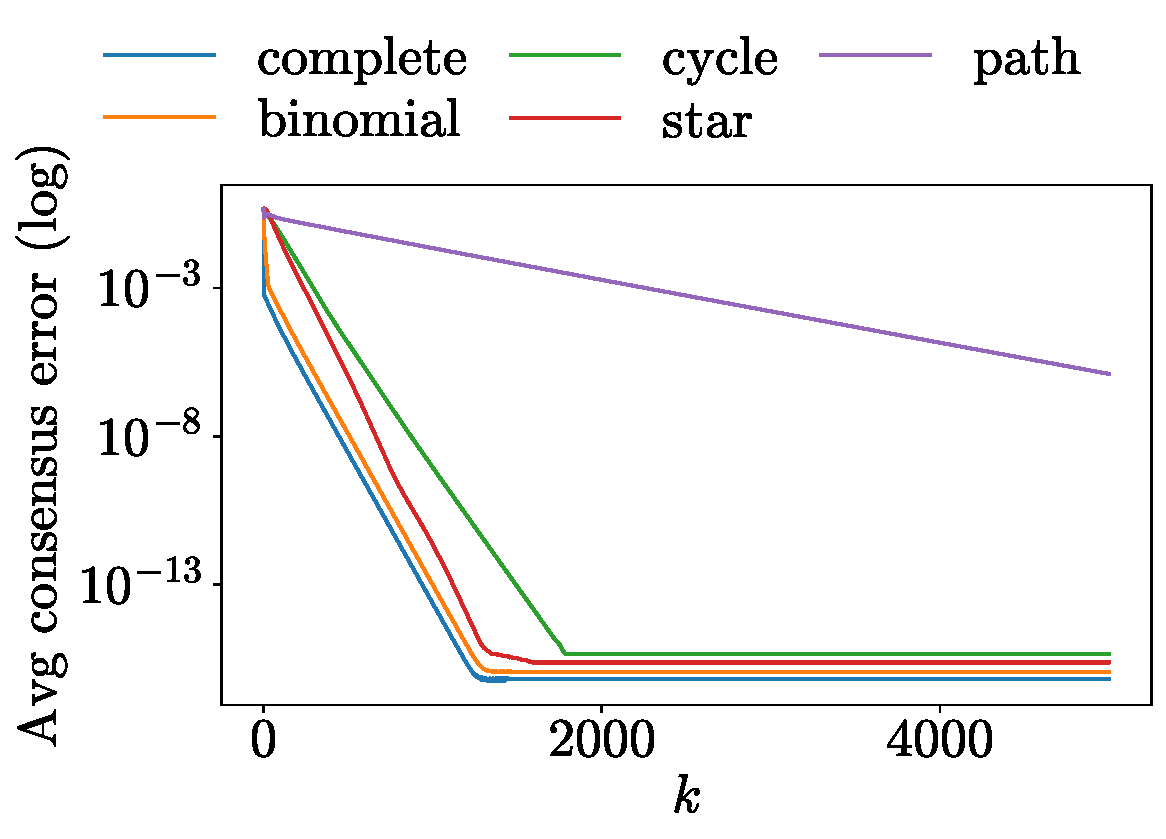
\includegraphics[width=\linewidth]{./figs/quadratic/15_3/consensus.pdf} 
%       %       \caption{Consensus error}
%       % \end{subfigure}
%       \caption{Quadratic function minimization with $15$ agents in $\R^{3}$ to convergence}
%       \label{fig:quadratic_15_3_1000}
% \end{figure}


\subsection{Comparison with centralized gradient}

Following the previous results, we select the configuration using the complete graph for the comparison with the centralized gradient method. In \Cref{fig:quadratic_centralized_15_3}, we can observe the results with $15$ agents, but the overall behavior is the same for all configurations. It can be seen that, as one could expect, the centralized gradient method is faster to converge compared to a distributed algorithm as it has available all the global information and does not rely on estimates and information exchange with the neighbors.

\begin{figure}[H]
      \centering
      \begin{subfigure}[t]{0.46\linewidth}
            \centering
            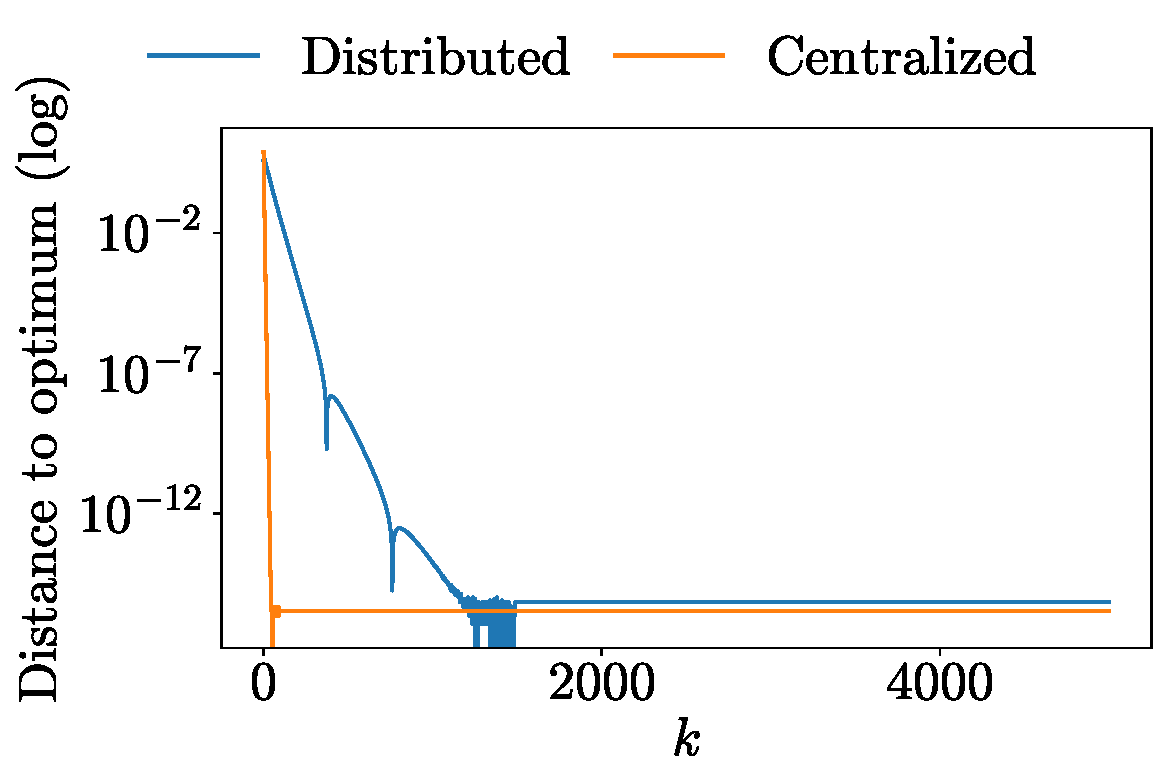
\includegraphics[width=\linewidth]{./figs/quadratic/centralized/distance.pdf} 
            \caption{Distance to optimum}
      \end{subfigure}
      \hfill
      \begin{subfigure}[t]{0.46\linewidth}
            \centering
            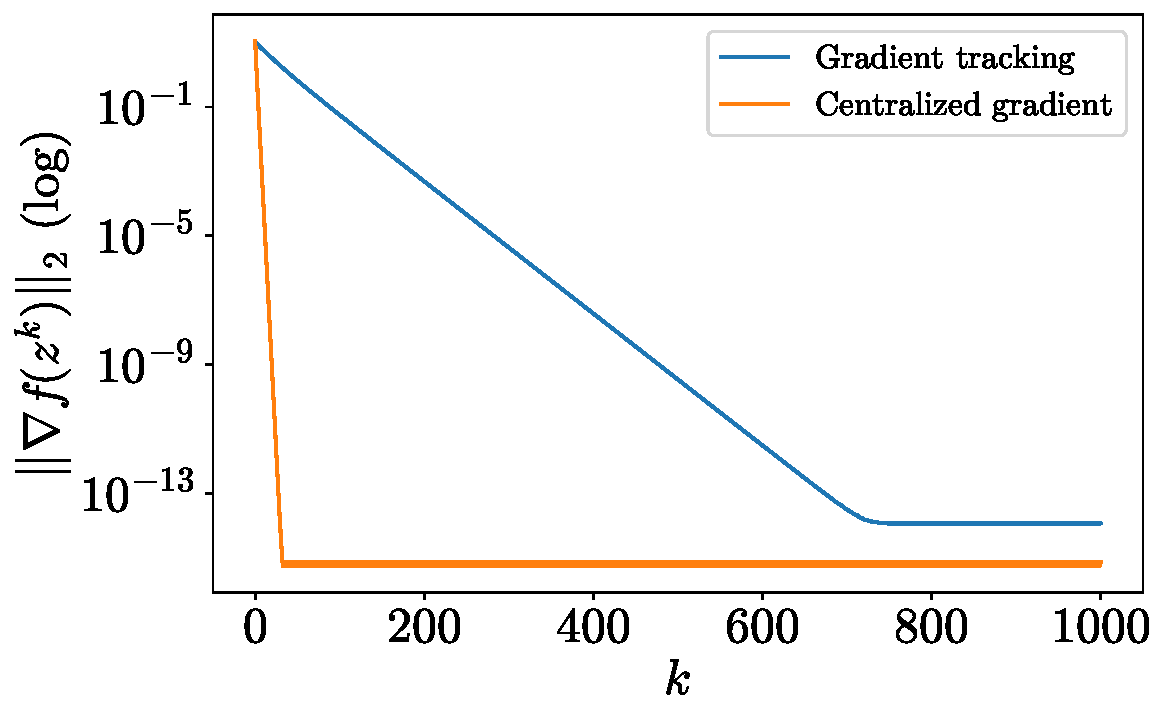
\includegraphics[width=\linewidth]{./figs/quadratic/centralized/gradient.pdf} 
            \caption{Gradient norm evolution}
      \end{subfigure}
      \caption{Quadratic function minimization with $15$ agents in $\R^{3}$ compared to centralized gradient}
      \label{fig:quadratic_centralized_15_3}
\end{figure}



\chapter{Cooperative multi-robot target localization} \label{ch:localization}


\section{Problem definition}

The problem in the second part of the first task involves a similar context as the previous case. The fundamental difference is that the local losses each agent has to minimize are designed to solve the problem of target localization. More specifically, this problem requires the implementation of a gradient tracking algorithm for estimating the position of $N_T$ fixed targets in a distributed way through $N_R$ tracking robots. Each robot is located at position $\p_i \in \R^2$ and it is assumed that the distance measured from each robot is noisy. Given the positions $\p_i$ and $\p_\tau$ of the $i$-th robot and the $\tau$-th target, respectively, we model the measured noisy distance $d_{i,\tau}$ as follows:
\[
      d_{i,\tau} = \Vert \p_i - \p_\tau \Vert + \varepsilon \cdot \texttt{noise}
\]
where $\texttt{noise} \sim P$ is drawn from some distribution $P$ and $\varepsilon \in \R$ is the noise rate.

The local loss each robot $i$ uses is the following:
\[
      \begin{gathered}
            l_i(\z) = \sum_{\tau=1}^{N_T} \left( d_{i,\tau}^2 - \Vert \z_{\tau} - \p_i \Vert^2 \right)^2
            \quad
            \nabla l_{i}(\z) = (\nabla l_{i,1}(\z_{1}), \dots, \nabla l_{i,N_T}(\z_{N_T}))
            \\
            \nabla l_{i,j}(\z_{j}) = -4 \left( d_{i,j}^2 - \Vert \z_{j} - \p_i \Vert^2 \right) \left( \z_{j} - \p_i \right)
      \end{gathered}
\]
where $\z = (\z_{\tau_1}, \dots, \z_{\tau_{N_T}}) \in \R^{2N_T}$ is the stack of decision variables of robot $i$ containing the estimated positions of the targets $\z_{\tau} \in \R^2$ and $\nabla l_i(\z) \in \R^{2N_T}$ is the concatenation of the gradients computed with respect to each target.

\section{Code structure}
The code provided is structured with the following main modules (considering only the ones which have differences with the previous case):
\begin{description}
      \item[loss.py] Class definition of the target localization loss function.
      \item[plot.py] All the functions used to plot the loss, gradient norm evolution over iterations.
      \item[scenarios.py] Two functions, one aiming to create the graph $G$ and the relative adjacency matrix $A$, while the other is designed to initialize the parameters (e.g., the ground truth target positions, initial robot positions, and noisy estimated target distances) and the target localization loss functions.
\end{description}
In practice all the experiments can be executed from the script \texttt{main\_tracking.py}.

\section{Experiments}

We approach the experimentation of such algorithm by trying different graph patterns and comparing with the centralized gradient method, similarly to the previous case. At first, we evaluated the performance of the algorithm in the following cases, all with the same type of noise:
\begin{itemize}
      \item Network of 5 robots and 1 target,
      \item Network of 5 robots and 3 targets, and
      \item Network of 15 robots and 3 targets.
\end{itemize}

Then, the focus switched to observe how much the performance changes in terms of noise. By fixing the problem configuration, we experimented with varying Gaussian noises, Poisson noises, and noise rates.


\subsection{Comparison between different graph patterns}

In terms of graph pattern, we can observe from \Cref{fig:tracking_5_1} and \Cref{fig:tracking_5_3} that with the same number of robots and increasing number of targets, the number of iterations required to converge is roughly the same. This makes sense as each target is independent to the others and can be tracked in parallel.

\begin{figure}[H]
      \centering
      \begin{subfigure}[t]{0.46\linewidth}
            \centering
            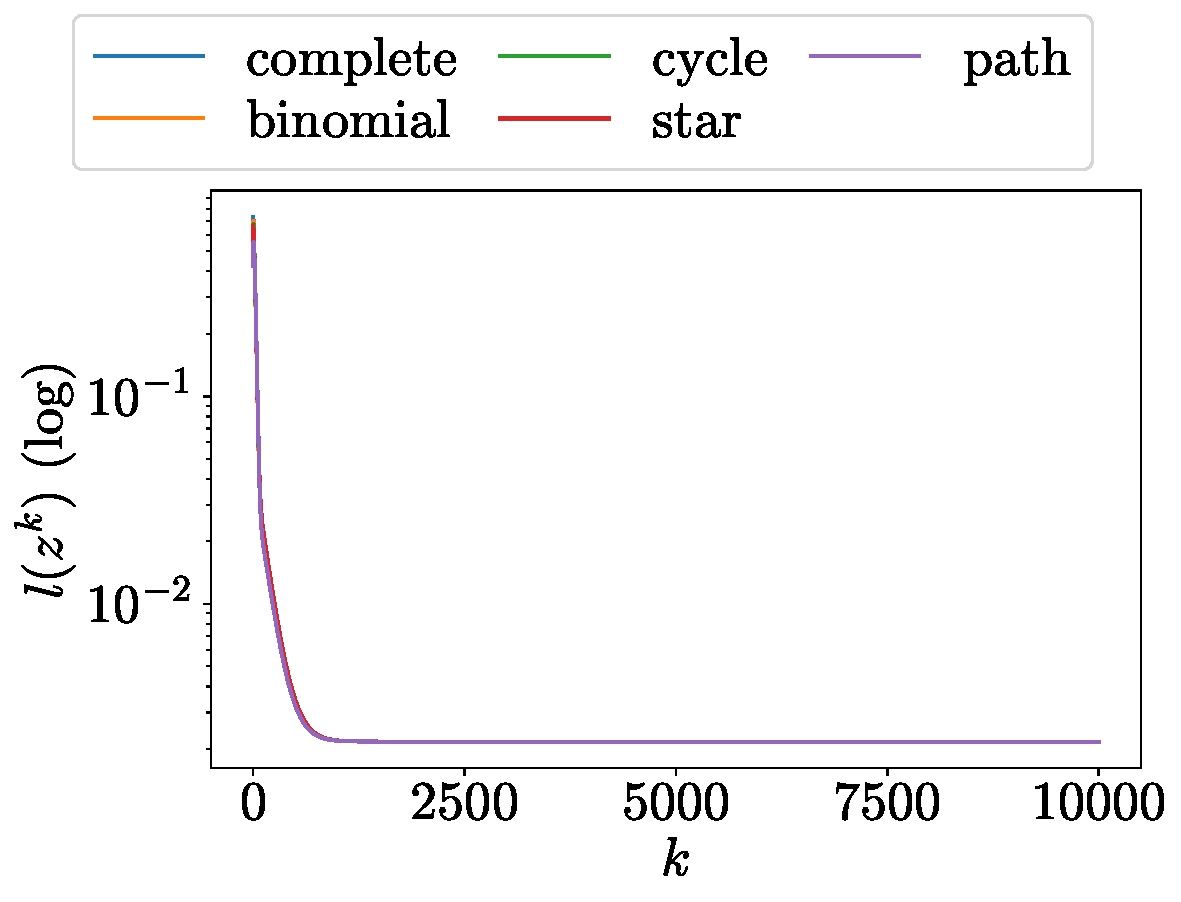
\includegraphics[width=\linewidth]{./figs/tracking/5_1_2/loss.pdf} 
            \caption{Loss evolution}
      \end{subfigure}
      \hfill
      \begin{subfigure}[t]{0.46\linewidth}
            \centering
            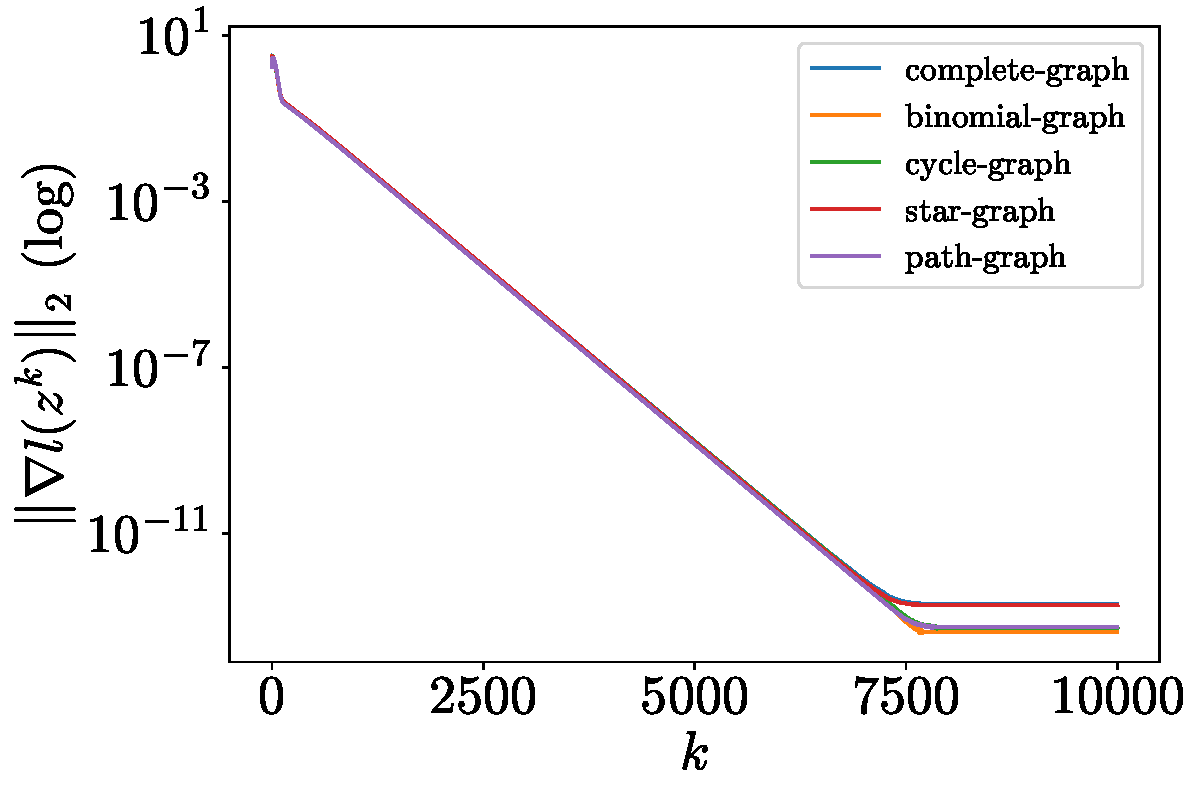
\includegraphics[width=\linewidth]{./figs/tracking/5_1_2/gradient.pdf} 
            \caption{Gradient norm evolution}
      \end{subfigure}
      \caption{Tracking with $5$ robots and $1$ target}
      \label{fig:tracking_5_1}
\end{figure}

\begin{figure}[H]
      \centering
      \begin{subfigure}[t]{0.46\linewidth}
            \centering
            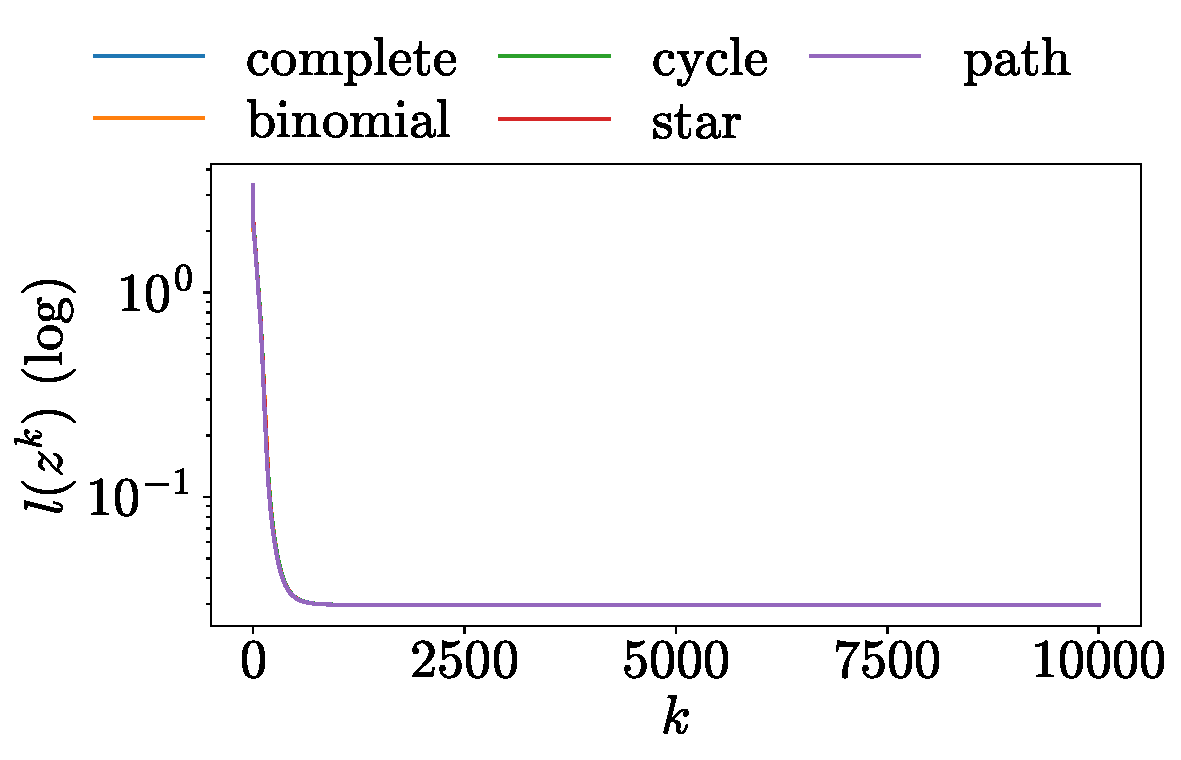
\includegraphics[width=\linewidth]{./figs/tracking/5_3_2/loss.pdf} 
            \caption{Loss evolution}
      \end{subfigure}
      \hfill
      \begin{subfigure}[t]{0.46\linewidth}
            \centering
            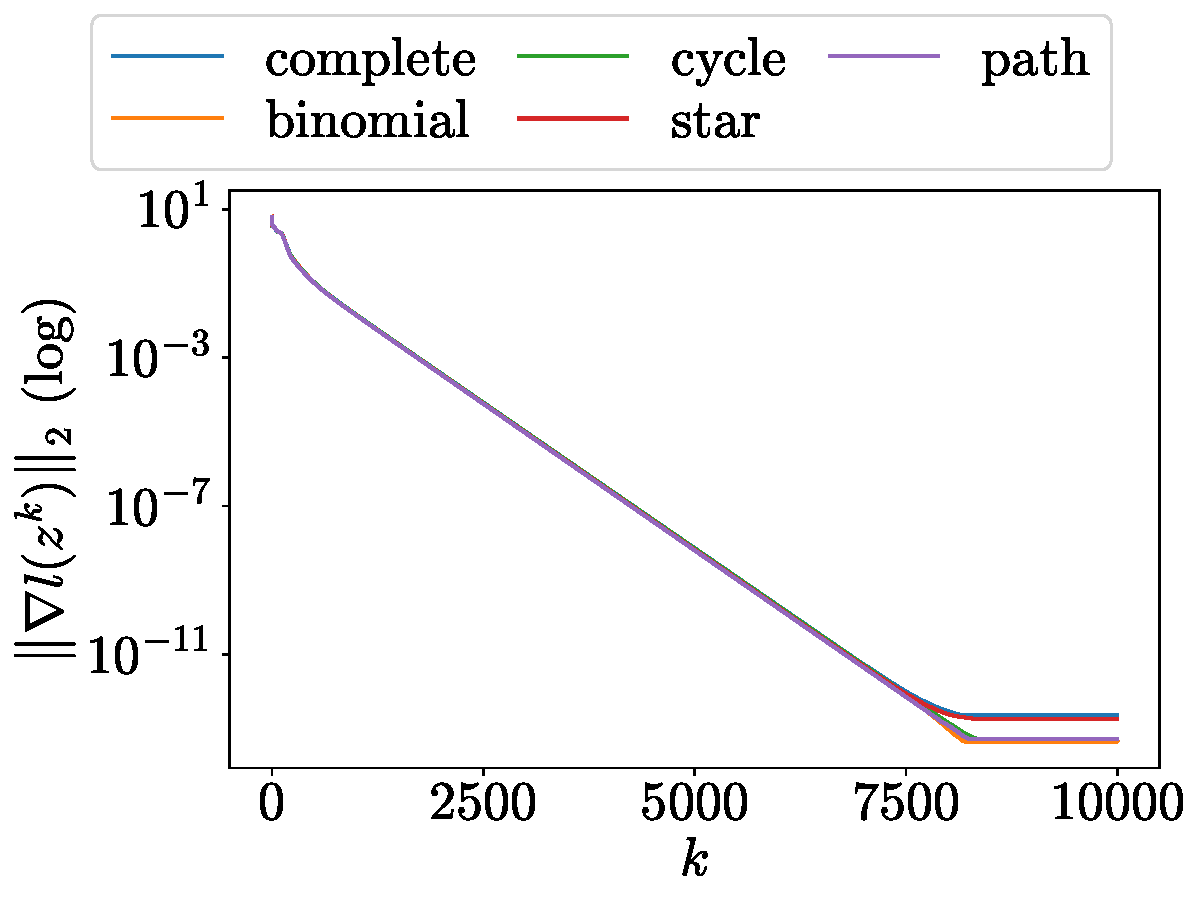
\includegraphics[width=\linewidth]{./figs/tracking/5_3_2/gradient.pdf} 
            \caption{Gradient norm evolution}
      \end{subfigure}
      \caption{Tracking with $5$ robots and $3$ targets}
      \label{fig:tracking_5_3}
\end{figure}

Instead, by increasing the number of tracking robots, we can see from \Cref{fig:tracking_15_3} that the plateau is reached in fewer number of iteration, which intuitively means that more tracking robots help in reaching a faster convergence.

\begin{figure}[H]
      \centering
      \begin{subfigure}[t]{0.46\linewidth}
            \centering
            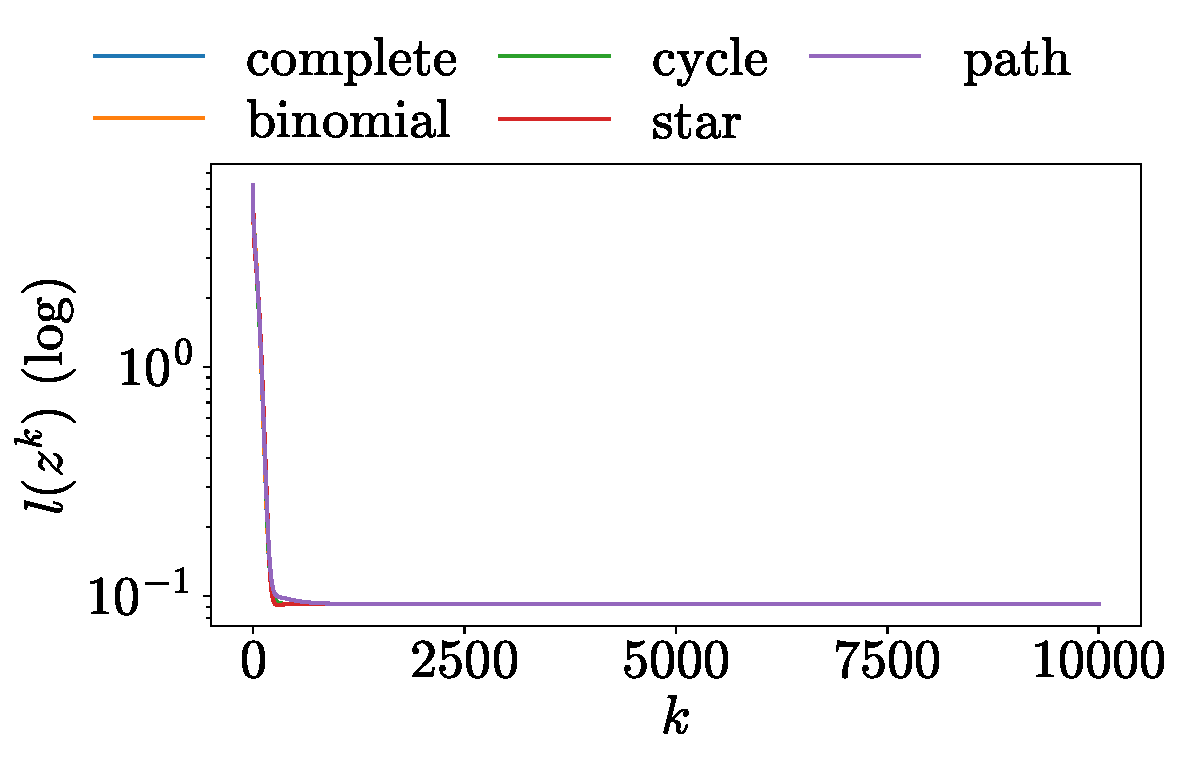
\includegraphics[width=\linewidth]{./figs/tracking/15_3_2/loss.pdf} 
            \caption{Loss evolution}
      \end{subfigure}
      \hfill
      \begin{subfigure}[t]{0.46\linewidth}
            \centering
            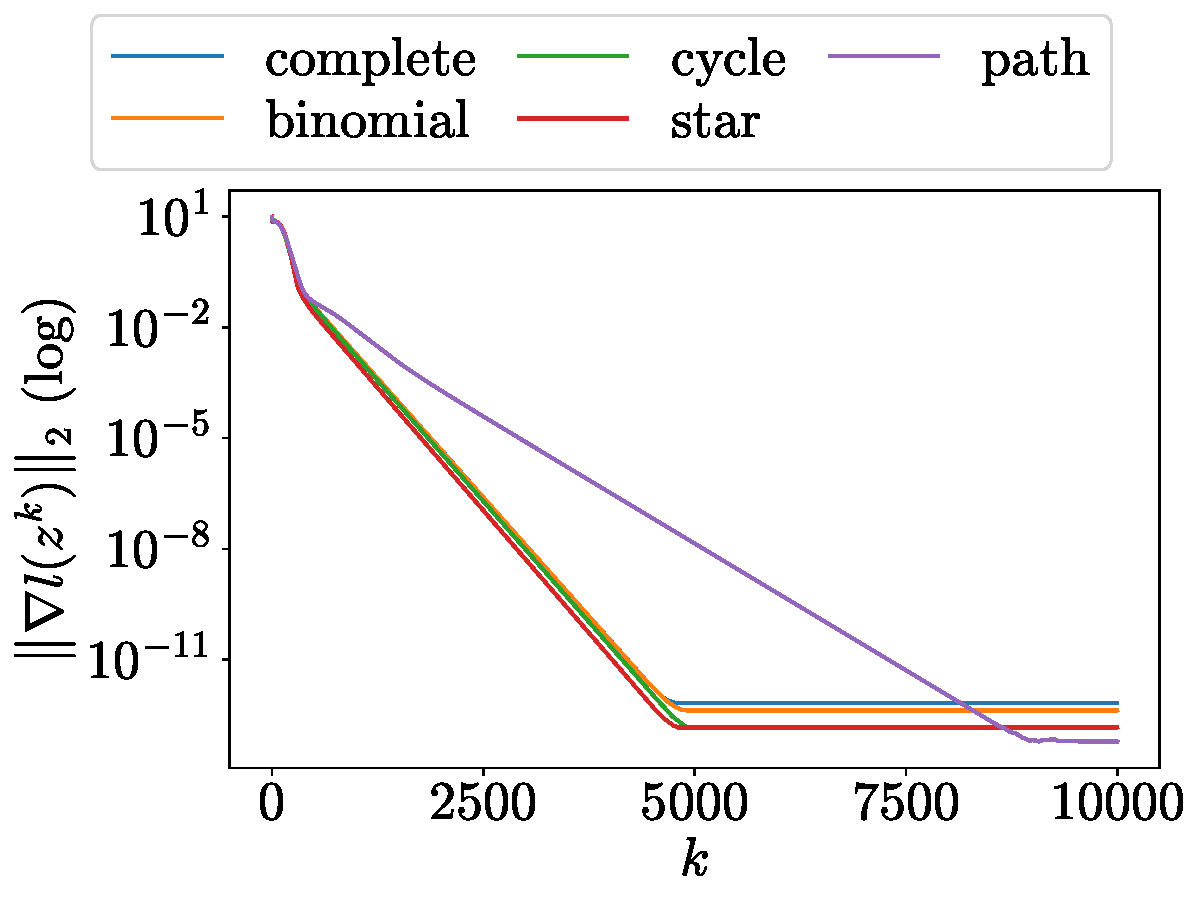
\includegraphics[width=\linewidth]{./figs/tracking/15_3_2/gradient.pdf} 
            \caption{Gradient norm evolution}
      \end{subfigure}
      \caption{Tracking with $15$ robots and $3$ targets}
      \label{fig:tracking_15_3}
\end{figure}

Moreover, as the total loss is a summation, we must note that the overall loss is higher in the case of more agents or targets, but this does not indicate worse tracking results. We report in \Cref{fig:tracking_avg_error_runs} the average distance between the estimated and real target positions for a fixed configuration with varying number of robots. It can be seen, as intuition would suggest, that on average the tracking error becomes smaller by increasing the number of tracking robots.

\begin{figure}[H]
      \centering
      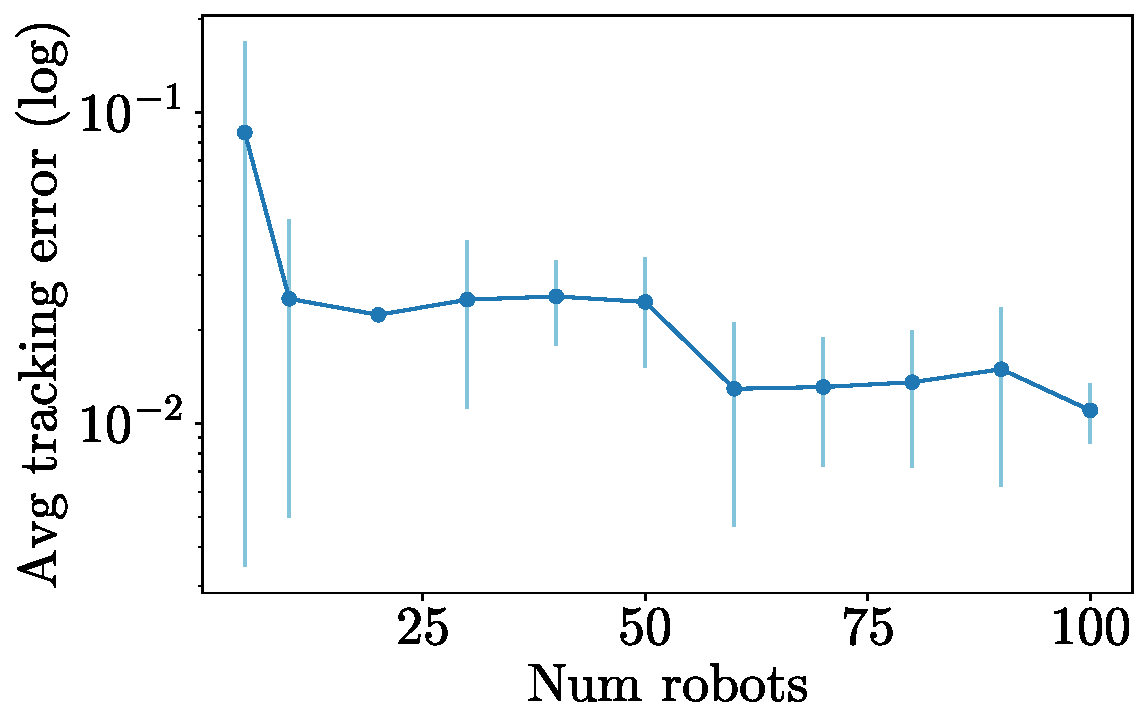
\includegraphics[width=0.46\linewidth]{./figs/tracking/average/avg_tracking.pdf}
      \caption{Average tracking error for different number of robots (average of 5 runs). Vertical bars represent the standard deviation.}
      \label{fig:tracking_avg_error_runs}
\end{figure}

% \begin{table}[ht]
%       \centering
%       \small
%       \caption{Average tracking error at the last iteration}
%       \label{tab:tracking_error}
%       \begin{tabular}{lccc}
%             \toprule
%             & $N_R=5, N_T=1$ & $N_R=5, N_T=3$ & $N_R=15, N_T=3$ \\
%             \midrule
%             \textbf{Complete} & $0.03008$ & $0.00554$ & $0.00500$ \\
%             \textbf{Binomial} & $0.03008$ & $0.00554$ & $0.00500$ \\
%             \textbf{Cycle}    & $0.03008$ & $0.00554$ & $0.00500$ \\
%             \textbf{Star}     & $0.03007$ & $0.00554$ & $0.00500$ \\
%             \textbf{Path}     & $0.03009$ & $0.00553$ & $0.00501$ \\
%             \bottomrule
%       \end{tabulcar}
% \end{table}

Finally, an observation consistent in all experiments is that, as shown in \Cref{fig:tracking_consensus}, the overall behavior of this system is to reach an approximate consensus (i.e., consensus error around $10^{-4}$) in the first few iterations and then optimize the loss while improving and preserving consensus. This can also be observed in \Cref{fig:tracking_animation} where a few frames of the animation of the scenario are shown.

\begin{figure}[H]
      \centering
      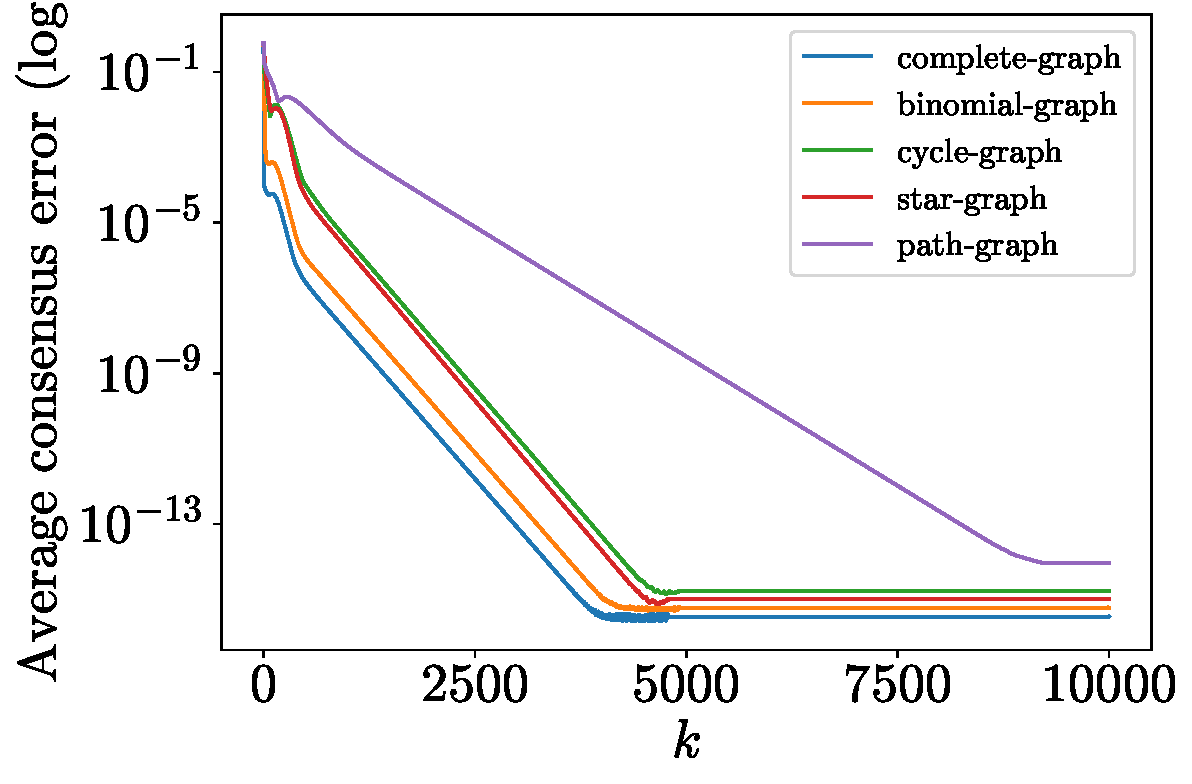
\includegraphics[width=0.46\linewidth]{./figs/tracking/15_3_2/consensus.pdf} 
      \caption{Tracking with $15$ robots and $3$ targets}
      \label{fig:tracking_consensus}
\end{figure}

\begin{figure}[H]
      \centering
      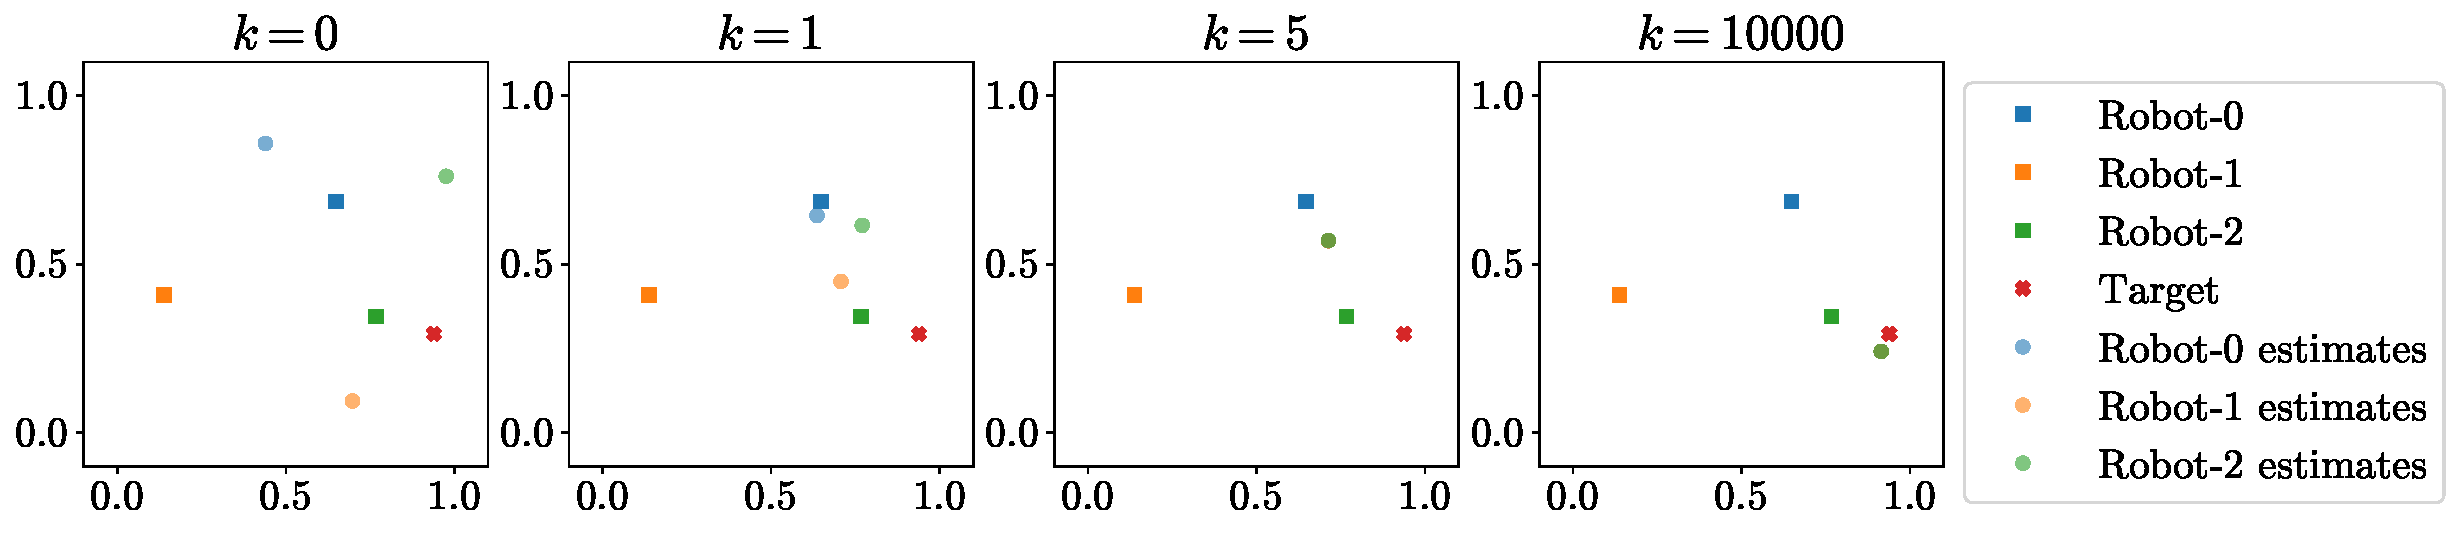
\includegraphics[width=\linewidth]{./figs/tracking/anim.pdf} 
      \caption{Tracking animation with $3$ robots and $1$ target}
      \label{fig:tracking_animation}
\end{figure}


\subsection{Comparison with centralized gradient}

Compared with the centralized gradient algorithm, the plots in \Cref{fig:tracking_centralized_5_3} confirm what we observed before in the case of quadratic functions. The convergence speed is faster and more accurate in a centralized approach, which also results in a lower average tracking error.

\begin{figure}[H]
      \centering
      \begin{subfigure}[t]{0.46\linewidth}
            \centering
            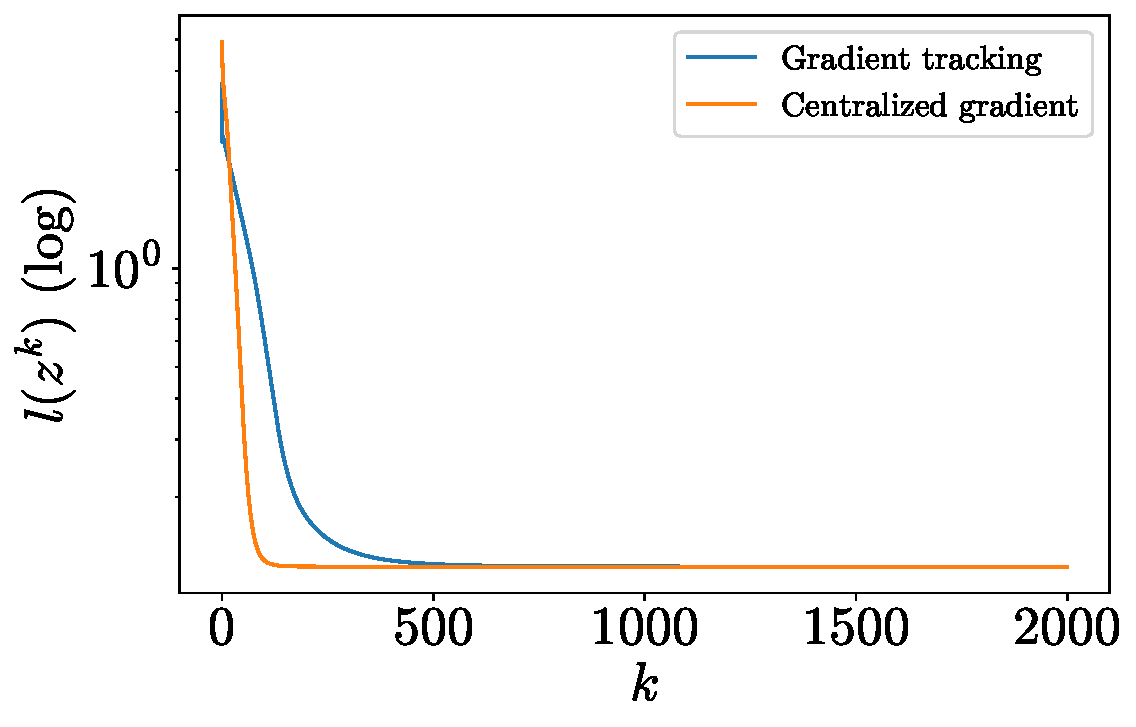
\includegraphics[width=\linewidth]{./figs/tracking/centralized/loss.pdf} 
            \caption{Loss evolution}
      \end{subfigure}
      \hfill
      \begin{subfigure}[t]{0.46\linewidth}
            \centering
            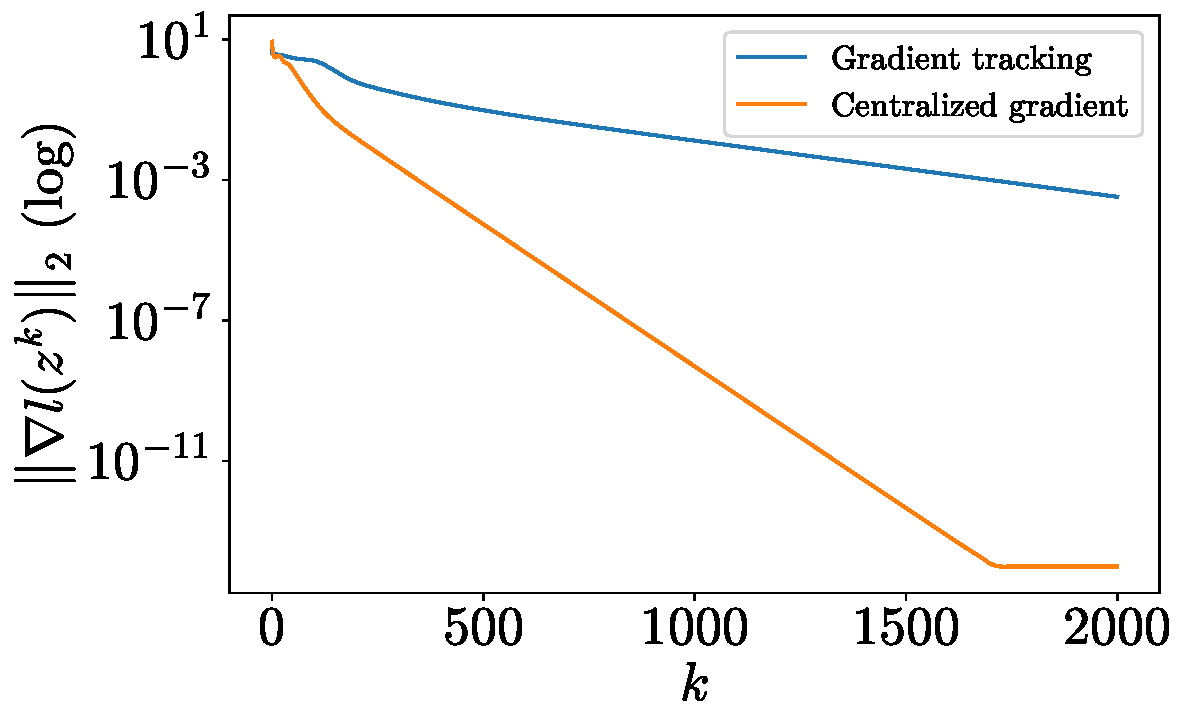
\includegraphics[width=\linewidth]{./figs/tracking/centralized/gradient.pdf} 
            \caption{Gradient norm evolution}
      \end{subfigure}
      \caption{Tracking with $15$ robots and $3$ targets with centralized gradient}
      \label{fig:tracking_centralized_5_3}
\end{figure}


\subsection{Different noises}

From the experiments with different noises, we observed a worsening in performance that is proportional to the amount of noise injected into the distance measurement, implying as one could expect that more noise leads to worse results. This behavior is consistent with noise drawn from different distributions as in \Cref{fig:tracking_gaussian_15_3} and \Cref{fig:tracking_poisson_15_3}, and also when the noise rate is increased as in \Cref{fig:tracking_rates_15_3}.

\begin{figure}[H]
      \centering
      \begin{subfigure}[t]{0.46\linewidth}
            \centering
            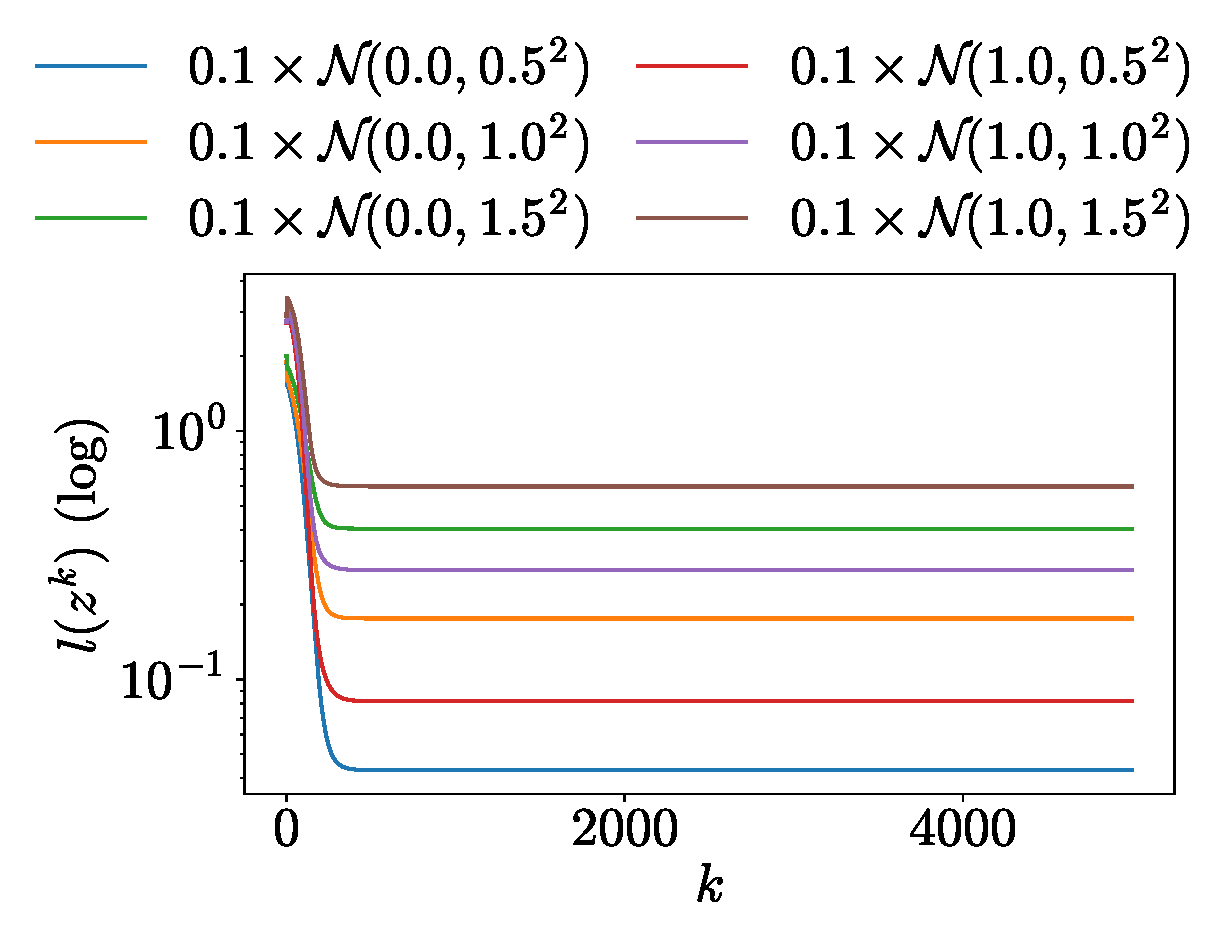
\includegraphics[width=\linewidth]{./figs/tracking/gaussian/loss.pdf} 
            \caption{Loss evolution}
      \end{subfigure}
      \hfill
      \begin{subfigure}[t]{0.46\linewidth}
            \centering
            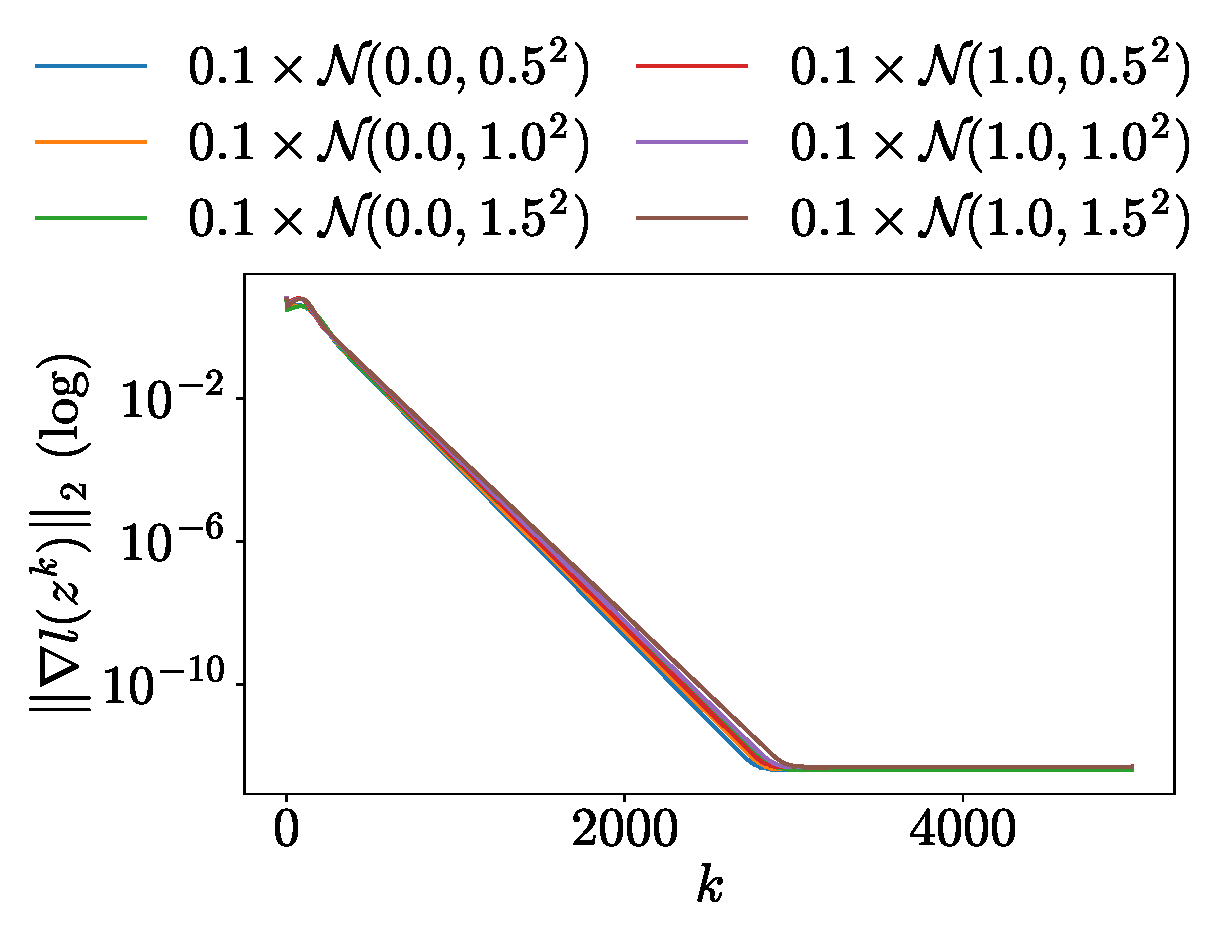
\includegraphics[width=\linewidth]{./figs/tracking/gaussian/gradient.pdf} 
            \caption{Gradient norm evolution}
      \end{subfigure}
      \caption{Tracking with $15$ robots and $3$ targets with noise drawn from Gaussian distributions}
      \label{fig:tracking_gaussian_15_3}
\end{figure}

\begin{figure}[H]
      \centering
      \begin{subfigure}[t]{0.46\linewidth}
            \centering
            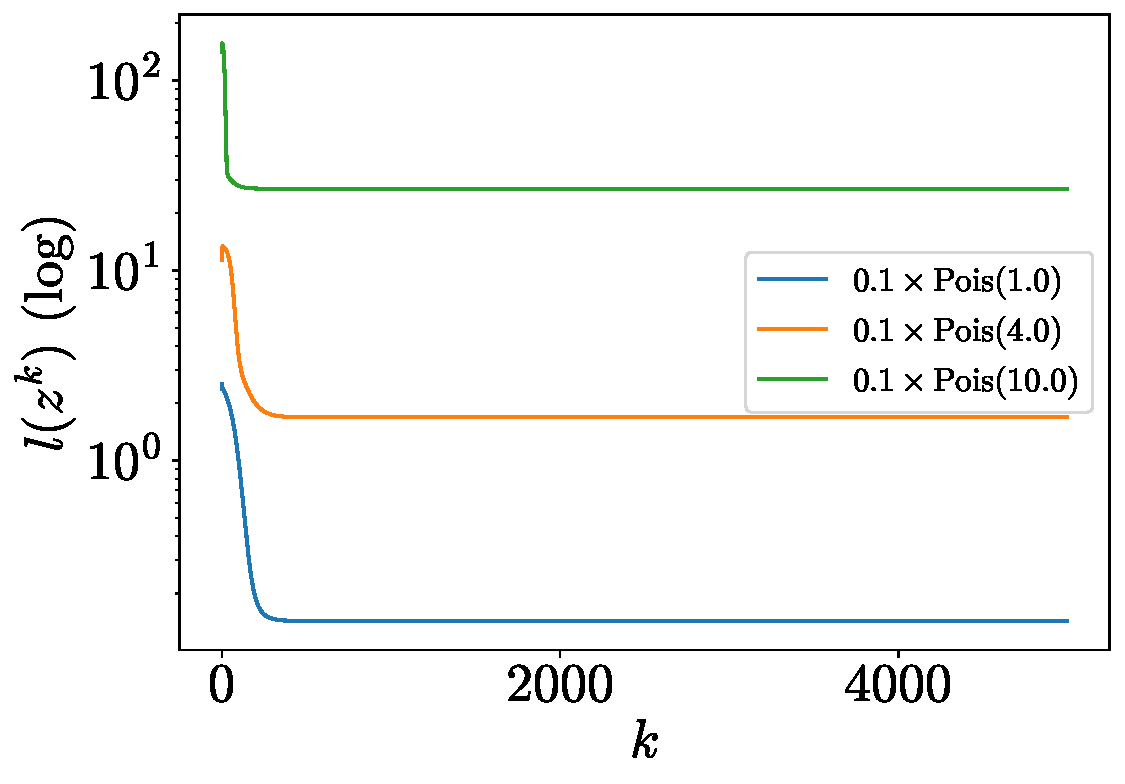
\includegraphics[width=\linewidth]{./figs/tracking/poisson/loss.pdf} 
            \caption{Loss evolution}
      \end{subfigure}
      \hfill
      \begin{subfigure}[t]{0.46\linewidth}
            \centering
            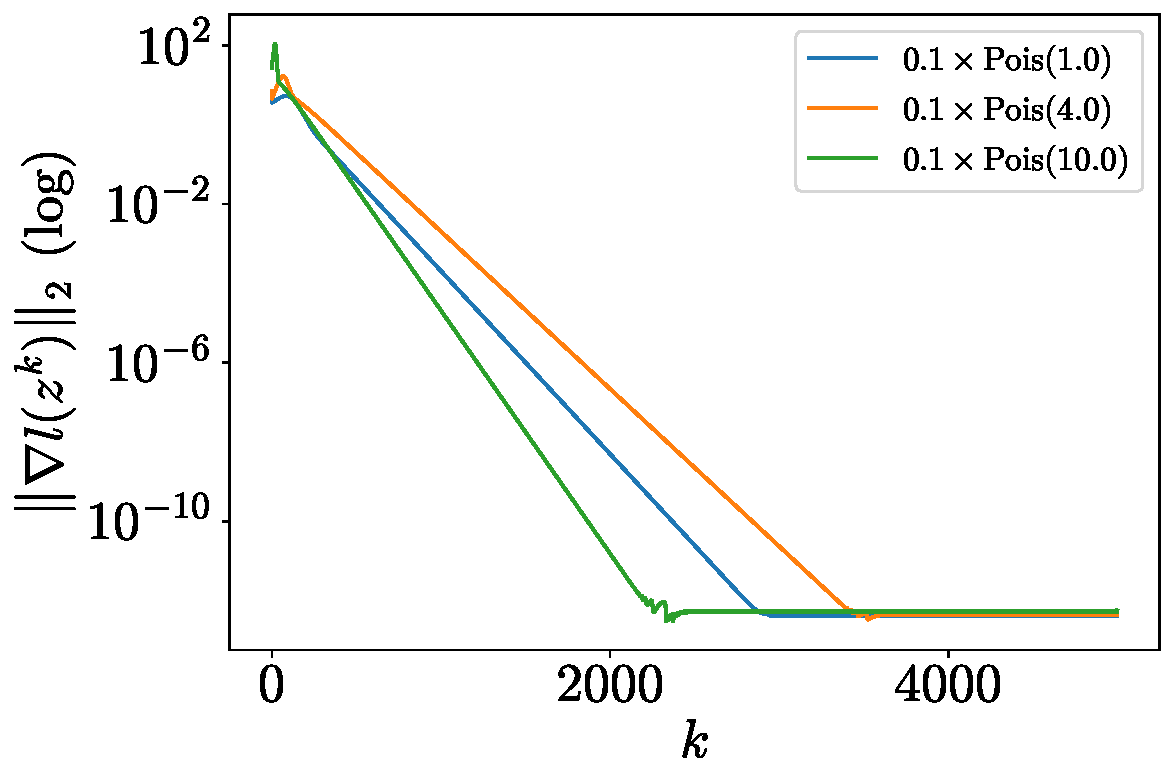
\includegraphics[width=\linewidth]{./figs/tracking/poisson/gradient.pdf} 
            \caption{Gradient norm evolution}
      \end{subfigure}
      \caption{Tracking with $15$ robots and $3$ targets with noise drawn from Poisson distributions}
      \label{fig:tracking_poisson_15_3}
\end{figure}

\begin{figure}[H]
      \centering
      \begin{subfigure}[t]{0.46\linewidth}
            \centering
            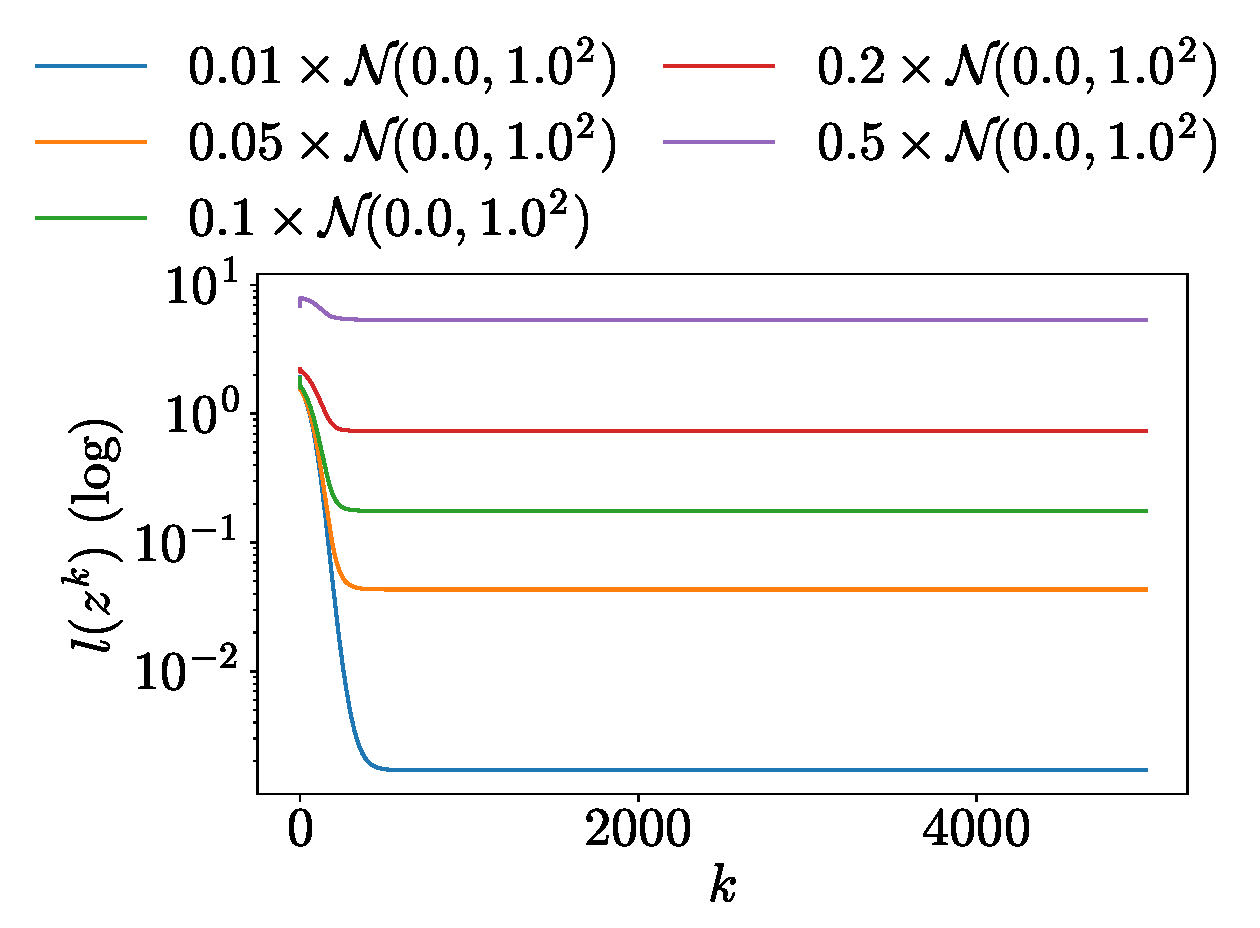
\includegraphics[width=\linewidth]{./figs/tracking/rates/loss.pdf} 
            \caption{Loss evolution}
      \end{subfigure}
      \hfill
      \begin{subfigure}[t]{0.46\linewidth}
            \centering
            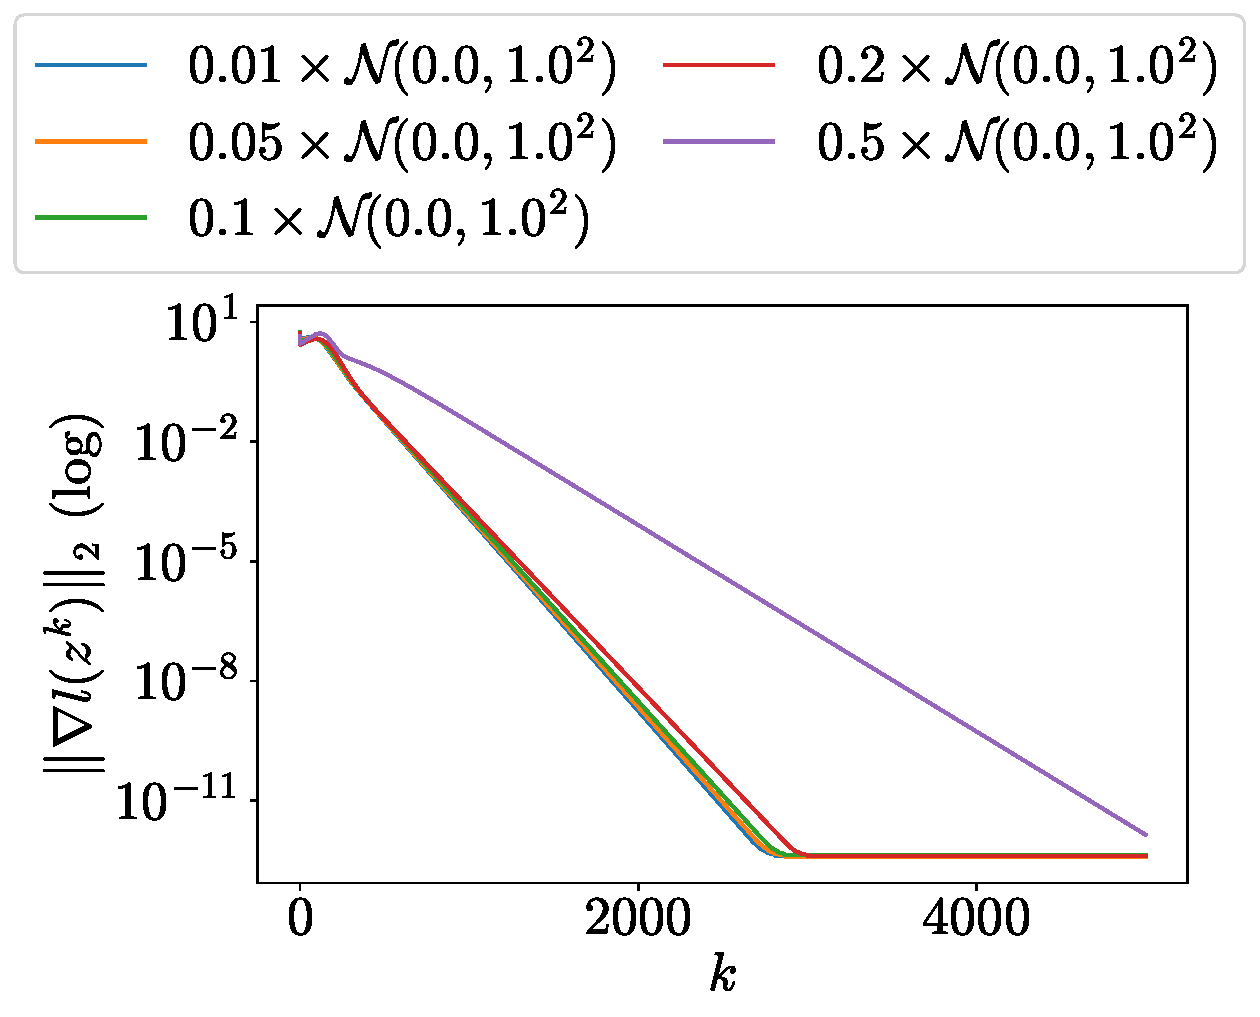
\includegraphics[width=\linewidth]{./figs/tracking/rates/gradient.pdf} 
            \caption{Gradient norm evolution}
      \end{subfigure}
      \caption{Tracking with $15$ robots and $3$ targets with different rates of Gaussian noise}
      \label{fig:tracking_rates_15_3}
\end{figure}




\chapter{Aggregative Optimization for Multi-Robot Systems} \label{ch:aggregative}


\section{Problem definition}

This task consists of solving the problem of moving $N \in \N$ agents with positions $\z_i \in R^2$ in such a way that they are close to their own private target $\r_i \in \R^2$ while staying tight to the fleet. This problem can be tackled using aggregative optimization by solving the following problem:
\[
      \begin{gathered}
            \min_{\z \in \R^{2N}} \sum_{i=1}^{N} l_i(\z_i, \sigma(\z)) \\
            \text{with } \sigma(\z) = \frac{1}{N} \sum_{i=1}^{N} \phi_i(\z_i),
      \end{gathered}
\]
where $\z=(\z_1, \dots, \z_N)$ is the stack of the agents' positions, $l_i: \R^2 \times \R^2 \rightarrow \R$ is the local losses of agent $i$ and $\sigma: \R^{2N} \rightarrow \R^2$ is an aggregation function.

We formulate the local loss of an agent $i$ as the following function:
\[
      l_i(\z_i, \sigma(\z)) = \gamma_1 \frac{1}{2} \Vert \z_i - \r_i \Vert^2 + \gamma_2 \frac{1}{2} \Vert \z_i - \sigma(\z) \Vert^2,
\]
where the first term models the vicinity to the private targets while the second one represents the fleet tightness. To add more flexibility, the hyperparameters $\gamma_1 \in \R$ and $\gamma_2 \in \R$ have been introduced to allow weighing the two requirements differently. The gradients of the loss with respect to the first and second arguments, respectively, are the following:
\[
      \begin{split}
            \nabla_1 l_i(\z_i, \sigma(\z)) &= \gamma_1 (\z_i - \r_i) + \gamma_2 (\z_i - \sigma(\z)) \\
            \nabla_2 l_i(\z_i, \sigma(\z)) &= -\gamma_2 (\z_i - \sigma(\z)),
      \end{split}
\]

In terms of aggregation function $\sigma(\z)$, the local function $\phi_i$ associated to each agent $i$ is defined as follows:
\[
      \phi_i(\z_i) = \alpha_i \z_i,
\]
where $\alpha_i \in R$ is a hyperparameter. With $\alpha_i = 1$ for all $i$, we obtain the standard formulation of the problem in which $\sigma(\z)$ represents the barycenter of the fleet. With different $\alpha_i$ (with $\sum_i^N \alpha_i = N$), we obtain a $\sigma(\z)$ that is a weighted average and can be interpreted as a barycenter that is biased towards specified agents.

\section{Code structure}
The code provided is structured with the following main modules:
\begin{description}
      \item[algorithm.py] Function implementing the aggregative optimization algorithm.
      \item[loss.py] Class definition of the Agent and its private functions, nominally the aggregative loss and the linear function needed to compute the barycenter.
      \item[plot.py] All the functions used to plot the loss, gradient norm evolution over iterations, but also an animation of the system and its single frames.
      \item[scenarios.py] Two functions, one aiming to create the graph $G$ and the relative adjacency matrix $A$, while the other designed to initialize the parameters for the problem (e.g., targets' positions and list of Agents).
\end{description}
TO DO: ROS2
In practice all the experiments can be executed from the script \texttt{main\_tracking.py}.

\section{Experiments}

As in the previous task, we first test the effectiveness of our implementation with different graph patterns for the communication graph and different number of agents. This aims at assessing convergence and scalability of the loss function. Then, to assess the actual results, we visually check the coherence of the positioning of the agents at convergence and experiment with different loss hyperparameters.


\subsection{Comparison with different graph patterns}

We first test the implementation with $5$ agents. From the plots in \Cref{fig:positioning_5}, we can observe an identical trend in terms of loss and gradient for every graph pattern we have experimented with. In all cases, we can observe that the algorithm converges, and also, visually, we can see that the final positions of the agents tends to reach an expected behavior.

By considering a scenario with $15$ agents, as shown in \Cref{fig:positioning_15}, we cannot detect any relevant changes in behavior as they all reach convergence in the same way as in the experiment with $5$ agents. The only thing we can underline is that the trend for the path graph has a little variation at convergence, most likely due to numerical instability.

\begin{figure}[H]
      \centering
      \begin{subfigure}[t]{0.46\linewidth}
            \centering
            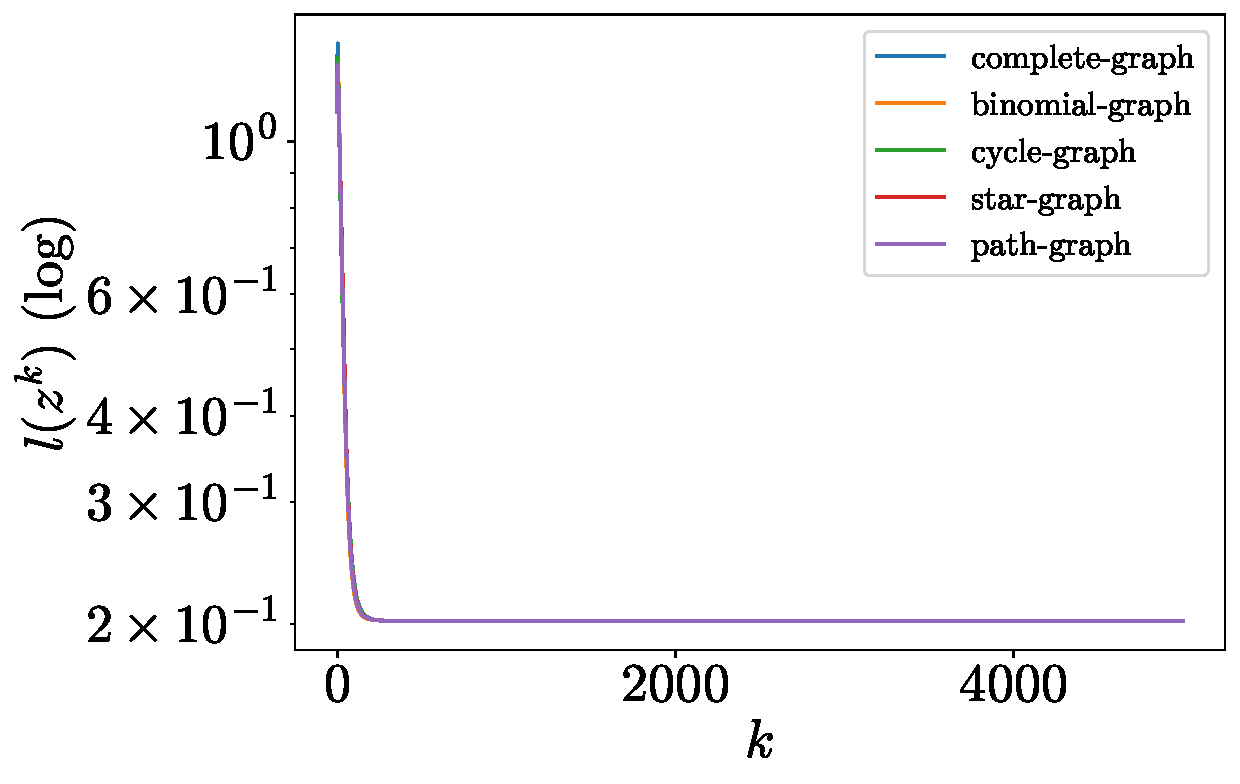
\includegraphics[width=\linewidth]{./figs/aggregative/few_agents/loss.pdf} 
            \caption{Loss evolution}
      \end{subfigure}
      \hfill
      \begin{subfigure}[t]{0.46\linewidth}
            \centering
            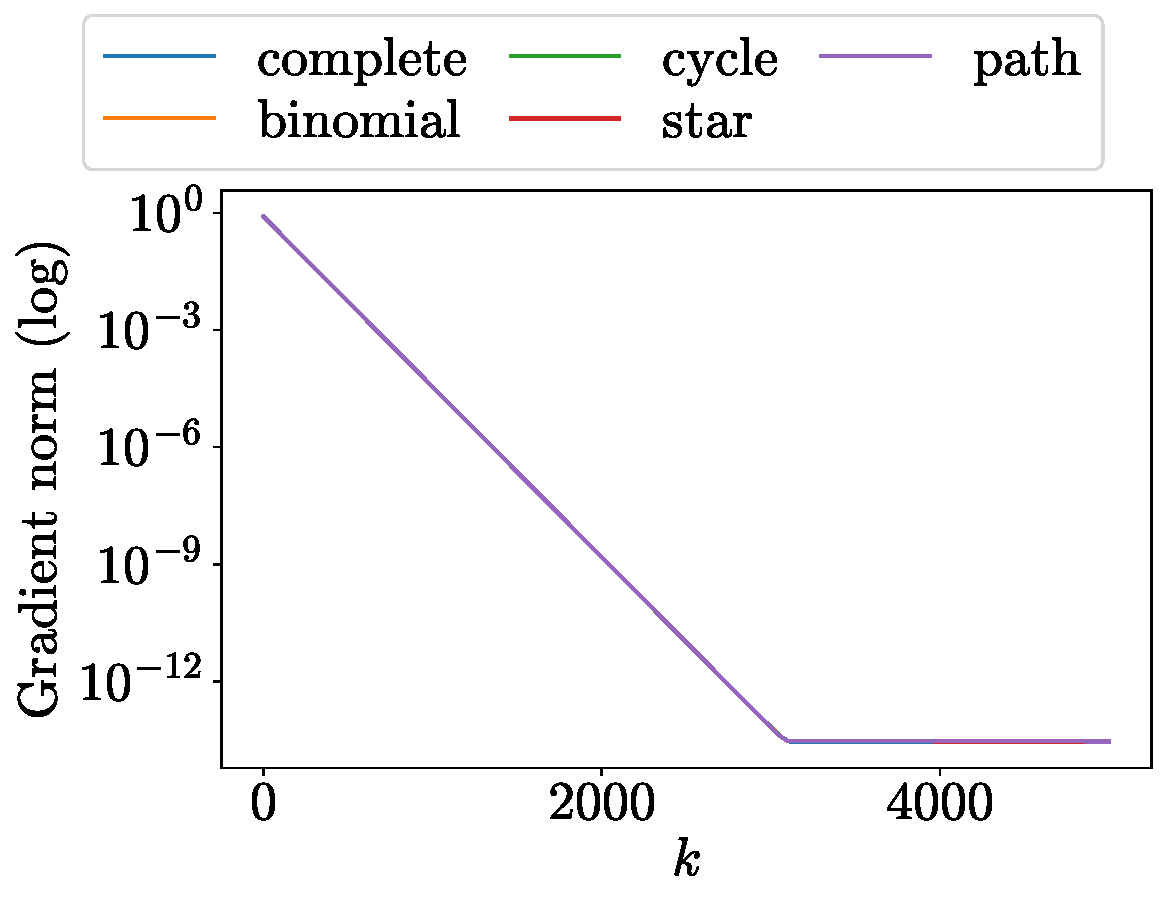
\includegraphics[width=\linewidth]{./figs/aggregative/few_agents/gradient.pdf} 
            \caption{Gradient norm evolution}
      \end{subfigure}
      \caption{Positioning with $5$ robots}
      \label{fig:positioning_5}
\end{figure}

\begin{figure}[H]
      \centering
      \begin{subfigure}[t]{0.46\linewidth}
            \centering
            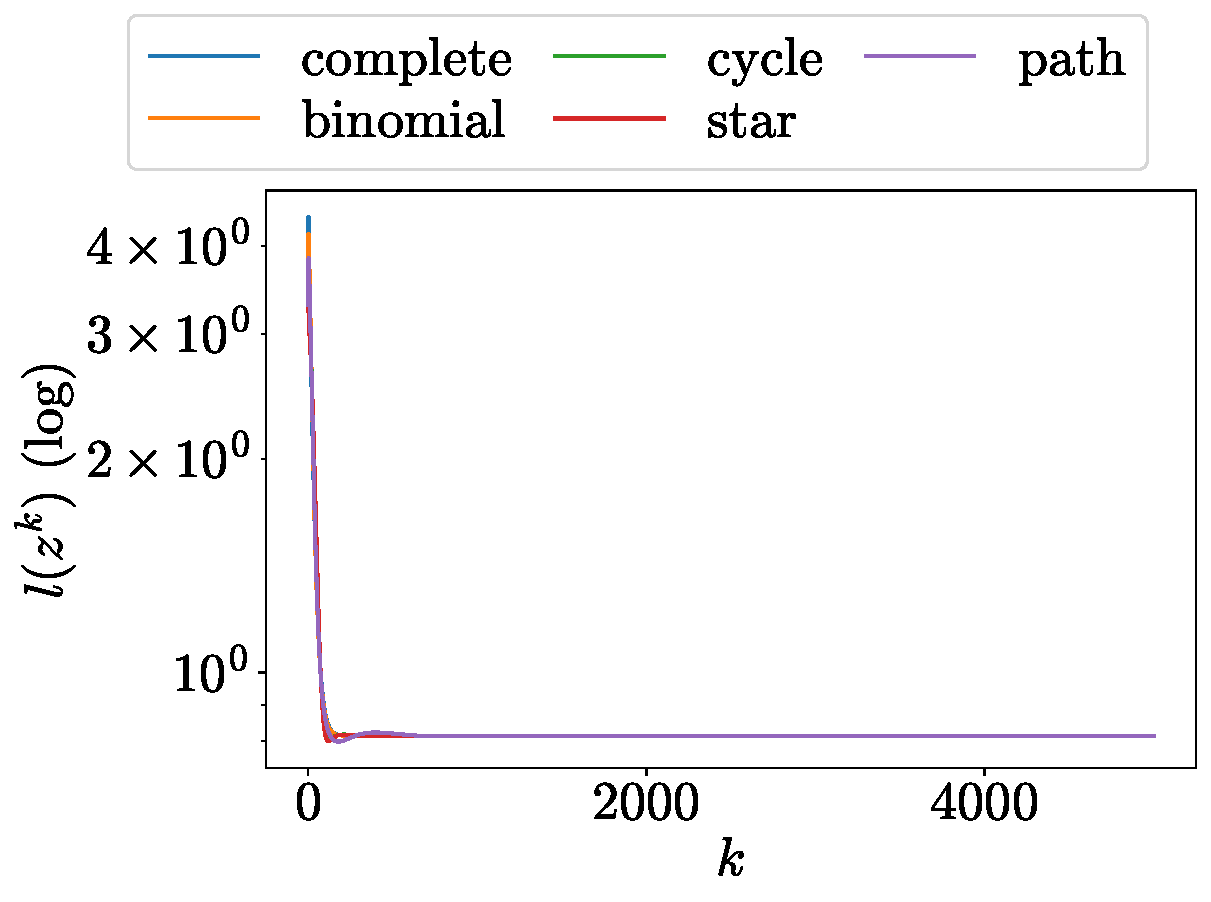
\includegraphics[width=\linewidth]{./figs/aggregative/more_agents/loss.pdf} 
            \caption{Loss evolution}
      \end{subfigure}
      \hfill
      \begin{subfigure}[t]{0.46\linewidth}
            \centering
            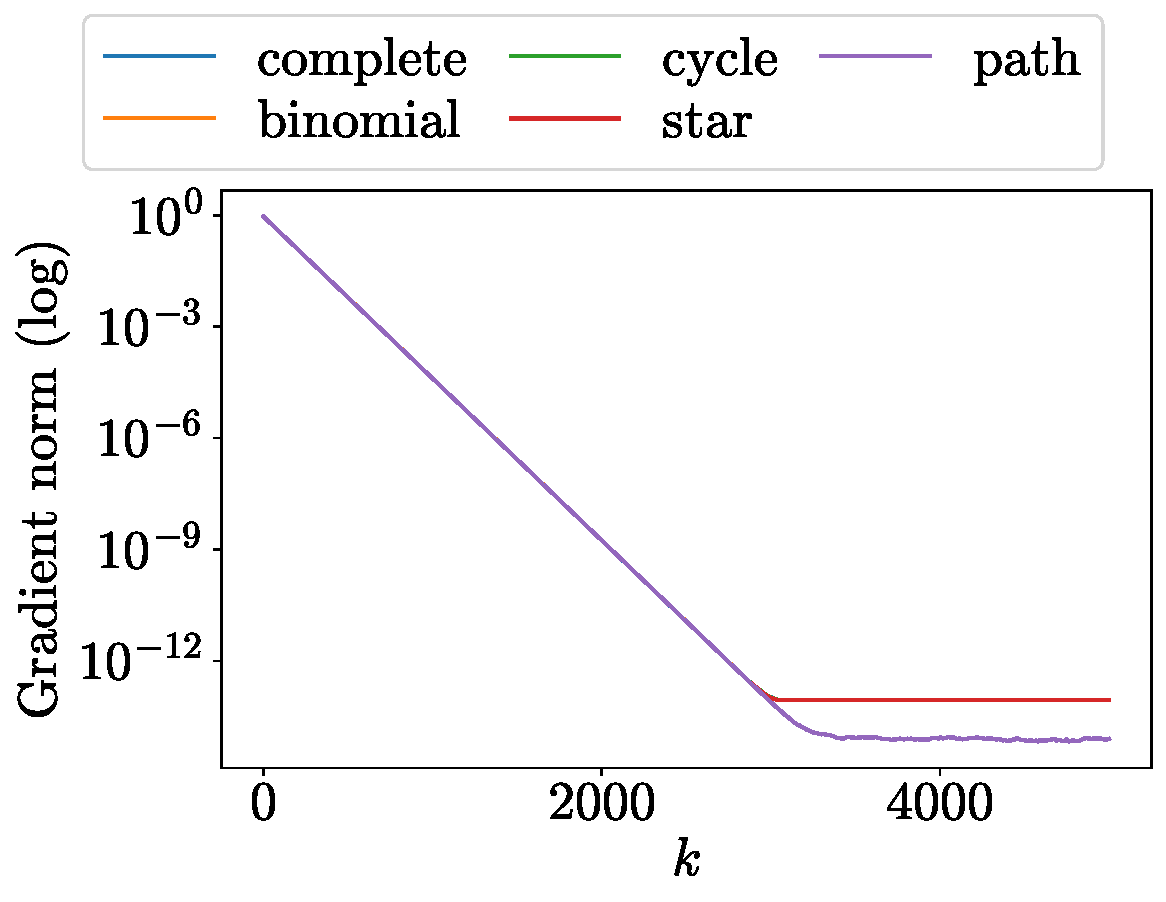
\includegraphics[width=\linewidth]{./figs/aggregative/more_agents/gradient.pdf} 
            \caption{Gradient norm evolution}
      \end{subfigure}
      \caption{Positioning with $15$ robots}
      \label{fig:positioning_15}
\end{figure}



\subsection{Comparison with different loss configurations}

To test the visual results, we first check the results in the plain version with equally weighted loss components and equal agents' importance. Results are presented in \Cref{fig:anim_plain}. As one could expect, with the two components of the loss balanced, the agents converge to a position that is midway between the barycenter and their private target.
\begin{figure}[H]
      \centering
      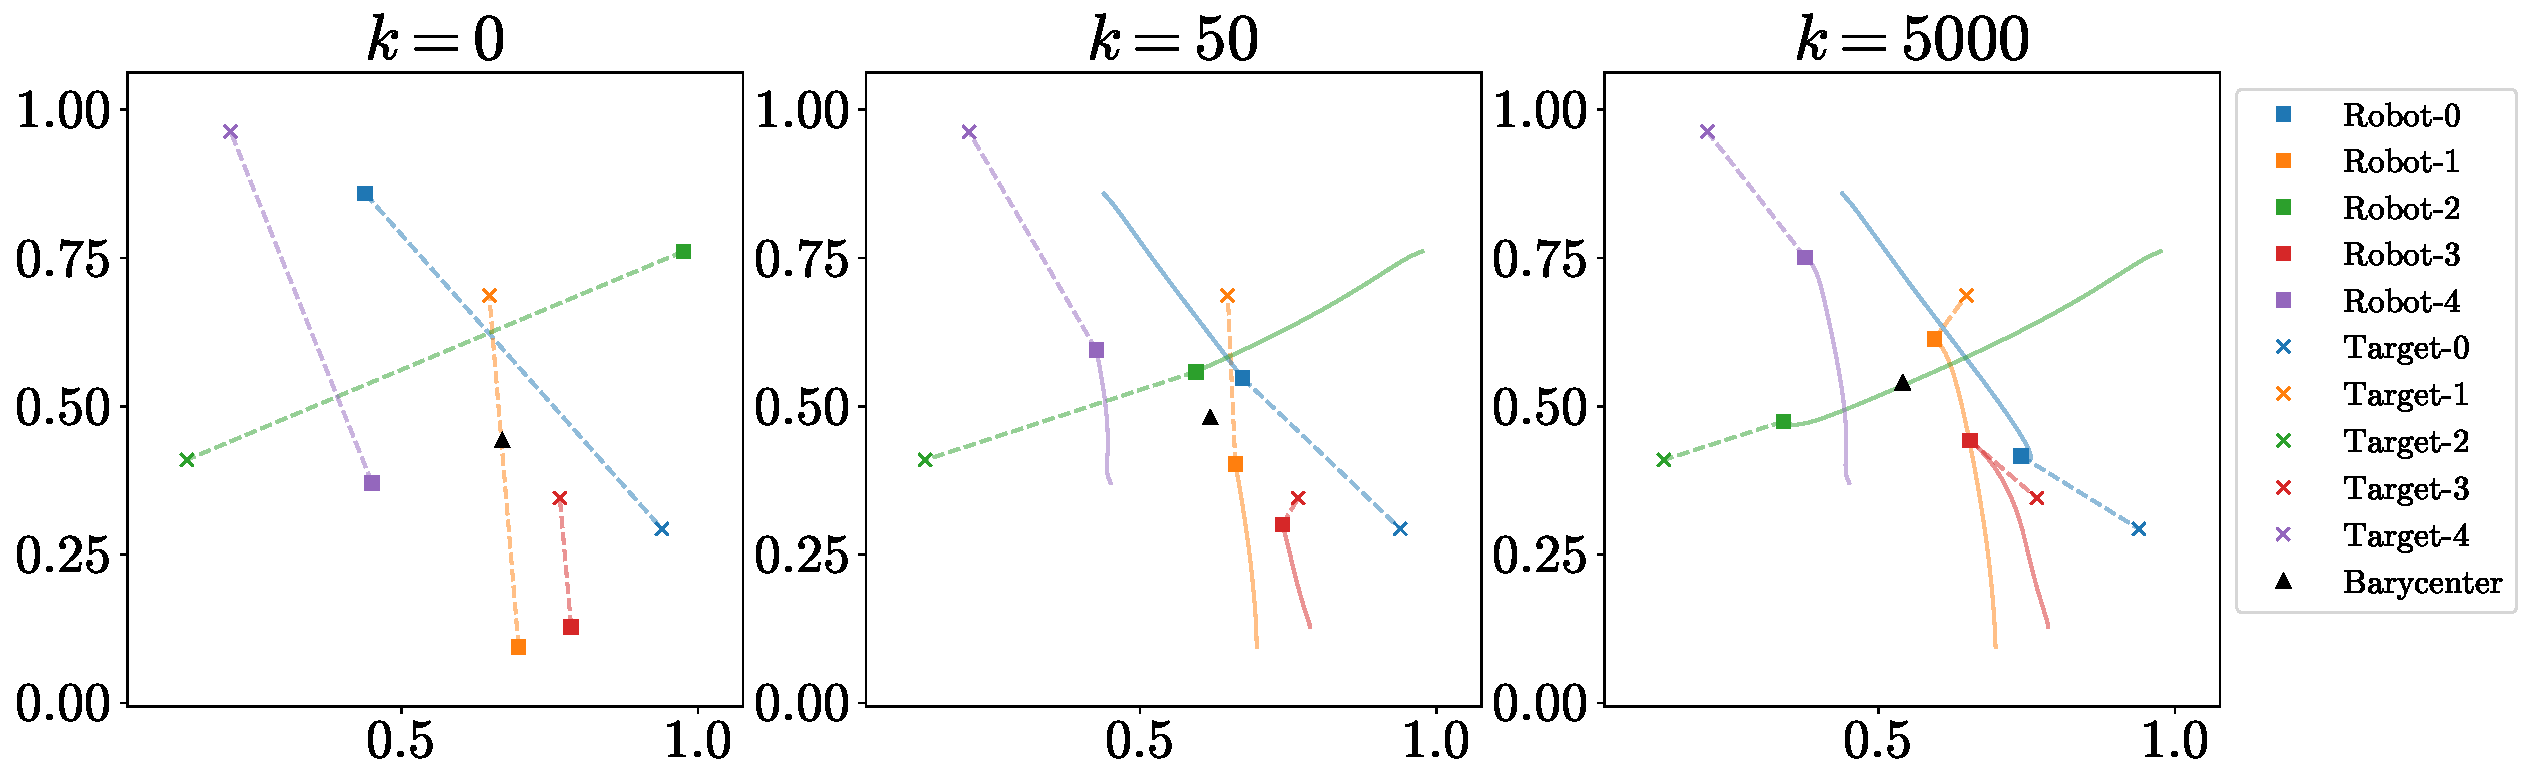
\includegraphics[width=0.9\linewidth]{./figs/aggregative/plain_anim/anim.pdf} 
      \caption{Frames with $5$ robots and balanced loss. Dashed lines connect robots to the targets and solid lines are the trajectories.}
      \label{fig:anim_plain}
\end{figure}

Then, we continue the experiments by checking the results in terms of different loss hyperparameters. We experiment our formulation with different weights to prioritize target vicinity (higher $\gamma_1$), barycenter vicinity (higher $\gamma_2$), and different agents' importance (different $\alpha_i$). Results are presented in \Cref{fig:anim_target}, \Cref{fig:anim_barycenter}, and \Cref{fig:anim_importance}, respectively. In all cases the positions at convergence are intuitively the expected ones, showing that the algorithm allows many degrees of freedom.




\begin{figure}[H]
      \centering
      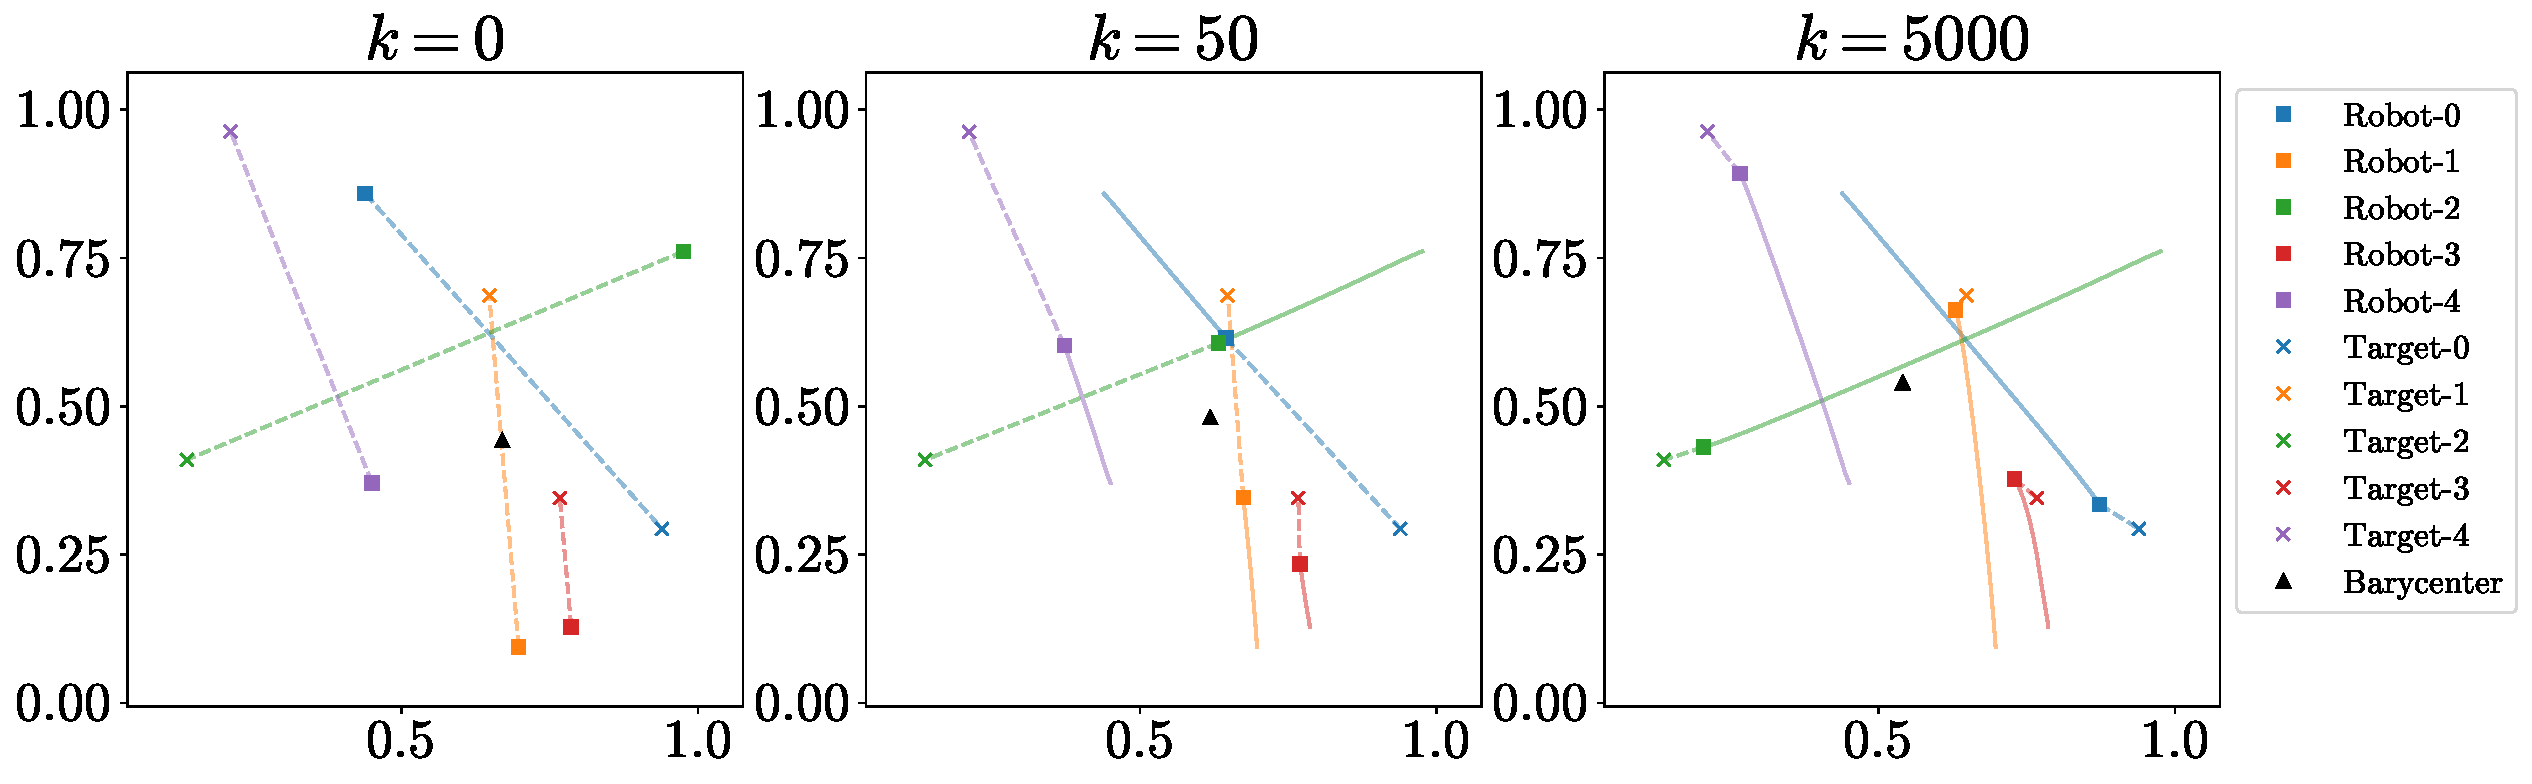
\includegraphics[width=0.9\linewidth]{./figs/aggregative/target_anim/anim.pdf} 
      \caption{Frames with $5$ robots and loss that prioritizes the private targets. Dashed lines connect robots to the targets and solid lines are the trajectories.}
      \label{fig:anim_target}
\end{figure}

\begin{figure}[H]
      \centering
      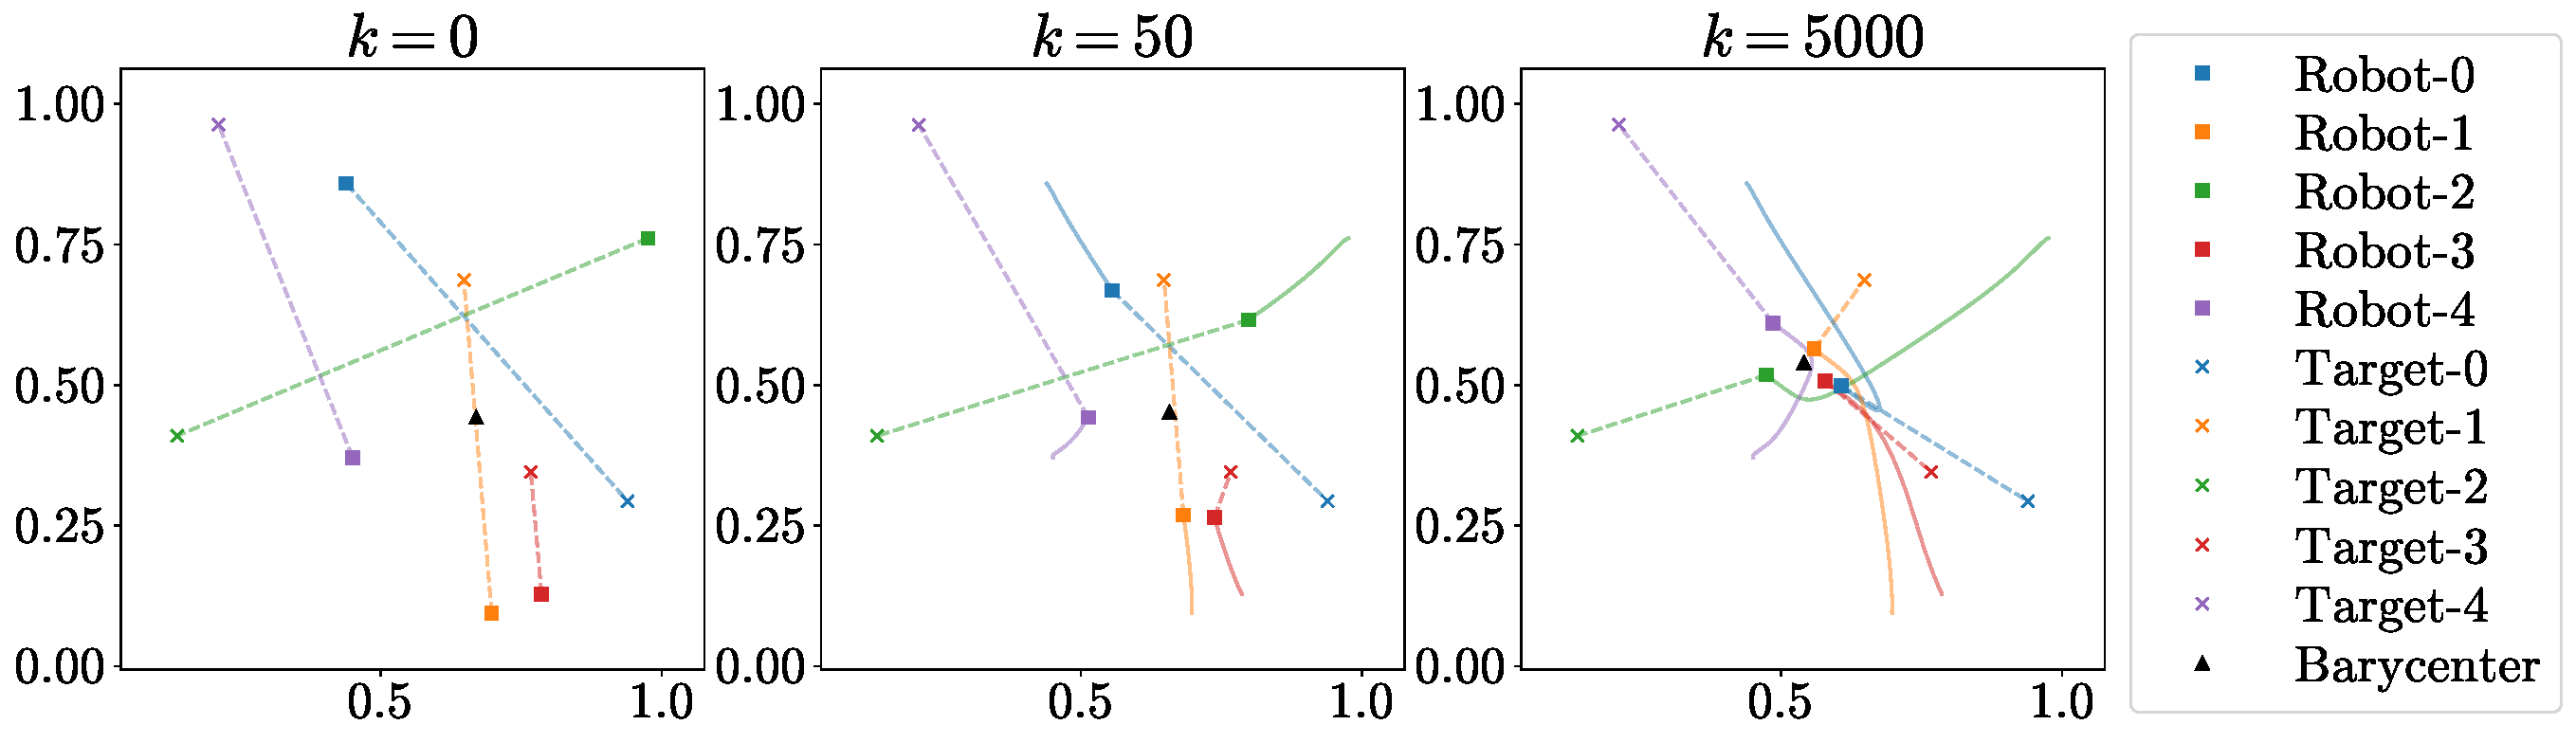
\includegraphics[width=0.9\linewidth]{./figs/aggregative/barycenter_anim/anim.pdf} 
      \caption{Frames with $5$ robots and loss that prioritizes the barycenter. Dashed lines connect robots to the targets and solid lines are the trajectories.}
      \label{fig:anim_barycenter}
\end{figure}

\begin{figure}[H]
      \centering
      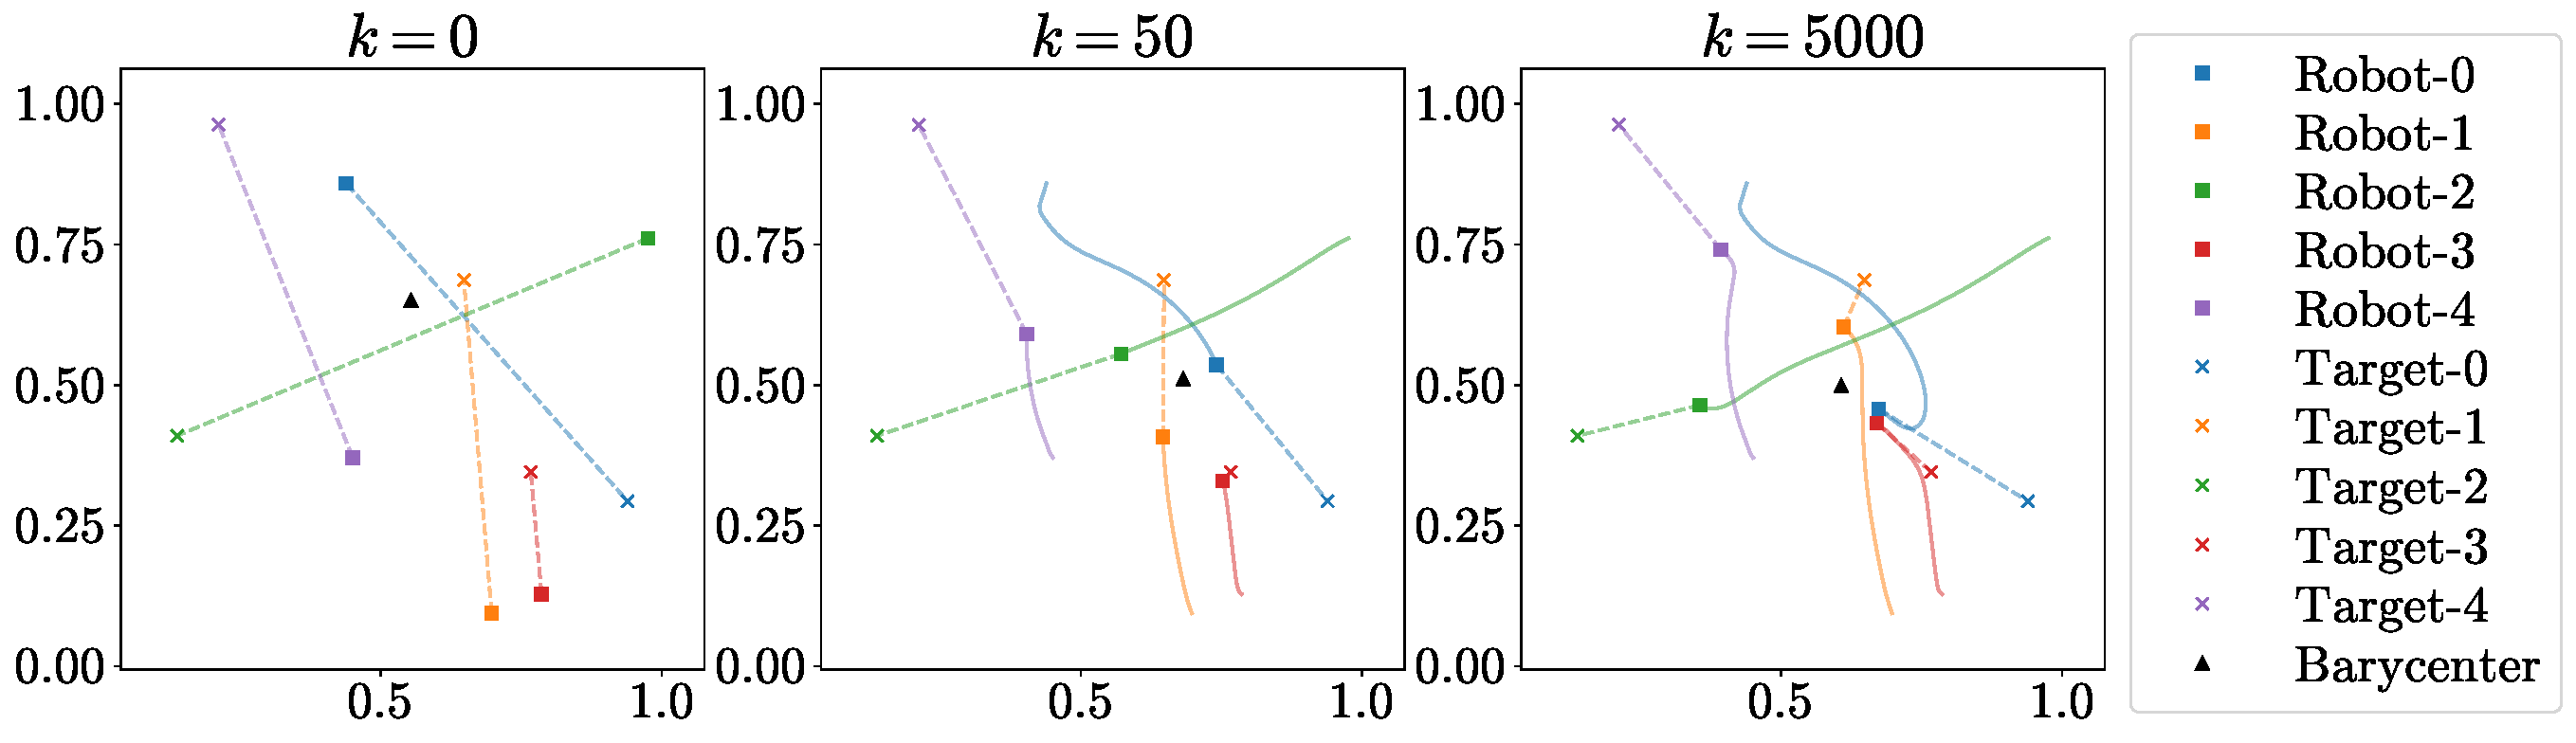
\includegraphics[width=0.9\linewidth]{./figs/aggregative/importance_anim/anim.pdf} 
      \caption{Frames with $5$ robots and barycenter that prioritizes robot $0$. Dashed lines connect robots to the targets and solid lines are the trajectories.}
      \label{fig:anim_importance}
\end{figure}



\chapter*{Conclusions}
\addcontentsline{toc}{chapter}{Conclusions} 

Both problems required for the first task and the second one were supported by a set of experiments. Within this paragraph we will show a summary of the results achieved.
Regarding the Multi-Robot Target Localization problem, we have performed a sequence of tests, which aim was to observe the variation of performance under different points of view. In particular, the loss and gradient norm evolution were evaluated over a varying number of agents and also in terms of dimensionality of the state variables. This test showed a nearly similar behavior for all kinds of graph patterns when using quadratic functions, with the only exception of the path graph, which was not able to reach convergence with an higher number of agents. This observation is most likely due to the fact that connectivity between agents in this case is very much relevant and that consequently the complexity of quadratic functions increase as well, requiring a greater number of iterations.
Instead, in the case of problem-specific loss function we were not able to denote relevant changes under the same circumstances. At most a faster convergence correlated to an higher number of agents.
Another test was executed to show how the algorithm behaves under different noise distributions and intensities. The outcome showed a linear relation between the obtained loss and the different parameters used in the definition of the noise distribution (for example, when using a Gaussian noise distribution the following parameters were considered: noise ratio, mean and standard deviation).
Regarding the Aggregative Optimization problem, we performed another sequence of tests to assess the change in behavior of the system and its performances. The first one aimed at observing how the loss and gradient norm evolution changed based on differents graph patterns. The outcome showed a nearly identical trend for all the configuration, independently of the increasing number of robots.
But also a set of loss hyperparameters were included in order to explore different behaviors. More specifically, we defined three parameters: agents' importance, targets' weights and barycenter's weights. The first one associated to each agent a real and positive coefficient, which contributed in the computation of the barycenter assigning more relevance to a particular agent instead of the others.
The second and the third one, simply injected more relevance to the target vicinity loss or to the barycenter vicinity loss by assigning an higher coeffincient to one or the other. 





% \bibliography{bibfile}{}


\end{document}